%% 
%% Author's note:
%% This was a template package which contains a lot of comments and code that were not written by me.
%%


%% Follow comments to support use.

%%%%%%%%%%%%%%%%%%%%%%%%%%%%%%%%%%%%%%%%%%%%%%%%%%%%%%%%%
%% STEP 1: Choose options for MSc / BSc / seminar layout and your bibliographic style
%%%%%%%%%%%%%%%%%%%%%%%%%%%%%%%%%%%%%%%%%%%%%%%%%%%%%%%%%

%%  Language: 
%%      finnish, swedish, or english
%%  Pagination (use twoside by default)  
%%      oneside or twoside,
%%  Study programme / kind of report
%%      csm  = Master's thesis in Computer Science Master's Programme;
%%      tkt = Bachelor's thesis in Computer Science Bachelor's Programme;
%%      seminar = seminar report
%%  For Master's thesis choose your line or track:
%%      (30 cr thesis, 2020 onwards, Master's Programme in Computer Science = csm)
%%      software-track-2020 = Software study track
%%      algorithms-track-2020 = Algorithms study track
%%      networking-track-2020 = Networking study track

\documentclass[english,twoside,censored,tkt]{HYthesisML} 

\widowpenalty=10000
\clubpenalty=10000


%% TODO: Check which is better (openright or openany).
% If wanted, open new chapters only at right page.
% By default, "openany".
%\PassOptionsToClass{openright,twoside,a4paper}{report}
\PassOptionsToClass{openany,twoside,a4paper}{report}

\usepackage{csquotes}
%%%%%%%%%%%%%%%%%%%%%%%%%%%%%%%%%%%%%%%%%%%%%%%%%%%%%%%%%
%% REFERENCES
%% Some notes on bibliography usage and options:
%% natbib -> you can use, e.g., \citep{} or \parencite{} for (Einstein, 1905); with APA \cite -> Einstein, 1905 without ()
%% maxcitenames=2 -> only 2 author names in text citations, if more -> et al. is used
%% maxbibnames=99 as no great need to suppress the biliography list in a thesis
%% for more information see biblatex package documentation, e.g., from https://ctan.org/pkg/biblatex 

%% Reference style: select one 
%% for APA = Harvard style = authoryear -> (Einstein, 1905) use:
\usepackage[style=authoryear,bibstyle=authoryear,backend=biber,natbib=true,maxnames=99,maxcitenames=2,uniquelist=minyear,giveninits=true,uniquename=mininit]{biblatex}
%% for numeric = Vancouver style -> [1] use:
%\usepackage[style=numeric,bibstyle=numeric,backend=biber,natbib=true,maxbibnames=99,giveninits=true,uniquename=init]{biblatex}
%% for alpahbetic -> [Ein05] use:
%\usepackage[style=alphabetic,bibstyle=alphabetic,backend=biber,natbib=true,maxbibnames=99,giveninits=true,uniquename=init]{biblatex}
%

\addbibresource{bibliography/articles.bib}  
\addbibresource{bibliography/books.bib}  
\addbibresource{bibliography/inproceedings.bib} 
\addbibresource{bibliography/reports.bib} 
% in case you want the final delimiter between authors & -> (Einstein & Zweistein, 1905) 
% \renewcommand{\finalnamedelim}{ \& }
% List the authors in the Bibilipgraphy as Lastname F, Familyname G,
\DeclareNameAlias{sortname}{family-given}
% remove the punctuation between author names in Bibliography 
%\renewcommand{\revsdnamepunct}{ }

% Asked chat.openai.com: I'm using biblatex package, but it prints odd format volume.number in reference list, while this should be volume (number). How to fix this?
%Answer (shortened):
% Redefine the volume and number format
%\DeclareFieldFormat[article]{volume}{\mkbibbold{#1}}
%\DeclareFieldFormat[article]{number}{\mkbibparens{#1}}
% Please remove the boldface from the volume and number fields:
\DeclareFieldFormat[article]{volume}{#1}
\DeclareFieldFormat[article]{number}{\mkbibparens{#1}}
% Now this generated format volume.(number). How to remove the dot? (and so on with some adjustments):
\renewbibmacro*{volume+number+eid}{%
  \setunit{\addcomma\space}% 
  \printfield{volume}%
  %\setunit*{\addnbspace\addthinspace}% <-- Adjust spacing here
  \printfield{number}%
  \setunit{\addcomma\space}%
  \printfield{eid}}


%% Block of definitions for fonts and packages for picture management.
%% In some systems, the figure packages may not be happy together.
%% Choose the ones you need.

%\usepackage[utf8]{inputenc} % For UTF8 support, in some systems. Use UTF8 when saving your file.

\usepackage{lmodern}         % Font package, again in some systems.
\usepackage{textcomp}        % Package for special symbols
\usepackage[pdftex]{color, graphicx} % For pdf output and jpg/png graphics
\usepackage{epsfig}
\usepackage{subfigure}
\usepackage[pdftex, plainpages=false]{hyperref} % For hyperlinks and pdf metadata
\usepackage{fancyhdr}        % For nicer page headers
\usepackage{tikz}            % For making vector graphics (hard to learn but powerful)
%\usepackage{wrapfig}        % For nice text-wrapping figures (use at own discretion)
\usepackage{amsmath, amssymb} % For better math
\usepackage{comment}
\usepackage{booktabs}
\usepackage{array}
\usepackage{tabularx}




\singlespacing               %line spacing options; normally use single

\fussy
%\sloppy                      % sloppy and fussy commands can be used to avoid overlong text lines
% if you want to see which lines are too long or have too little stuff, comment out the following lines
% \overfullrule=1mm
% to see more info in the detailed log about under/overfull boxes...
% \showboxbreadth=50 
% \showboxdepth=50



%%%%%%%%%%%%%%%%%%%%%%%%%%%%%%%%%%%%%%%%%%%%%%%%%%%%%%%%%
%% STEP 2:
%%%%%%%%%%%%%%%%%%%%%%%%%%%%%%%%%%%%%%%%%%%%%%%%%%%%%%%%%
%% Set up personal information for the title page and the abstract form.
%% Replace parameters with your information.
\title{AI-powered social engineering}


\author{Riku Talvisto}
\date{\today}
\newcommand{\thesisdate}{February 20, 2025}

% Set supervisors, use the titles according to the thesis language
% in English Prof. or Dr., or in Finnish toht. or tri or FT, TkT, Ph.D. or in Swedish... 
\supervisors{Docent Lea Kutvonen}

\keywords{social engineering, artificial intelligence, generative AI, cybersecurity, phishing, deepfake, ChatGPT}
%\additionalinformation{\translate{\track}}
\additionalinformation{}

%% For seminar reports:
%%\additionalinformation{Name of the seminar}

%% Provide classification terms, to appear on the abstract page.
%% Replace the classification terms below with the ones that match your work.
%% ACM Digital library provides a taxonomy and a tool for classification
%% in computer science. Use 1-3 paths, and use right arrows between the
%% about three levels in the path; each path requires a new line.

%% TODO: Which are most suitable? Should I include one, 2 or 3? Should I include the document type (surveys and overviews) and is that correct?
%% TODO: Should any title be in bold or any in italics?
\classification{\protect{\ \\
\  Social and professional topics $\rightarrow$ Computing / technology policy  $\rightarrow$ Computer crime \\ $\rightarrow$ \textbf{Social engineering attacks} \\
%%\  Human-centered computing $\rightarrow$ Collaborative and social computing  $\rightarrow$ Collaborative and social computing theory, concepts and paradigms $\rightarrow$ Social engineering (social sciences) \\
\  Security and privacy $\rightarrow$ Intrusion/anomaly detection and malware mitigation \\ $\rightarrow$ \textbf{Social engineering attacks}
}}

%% If you want to quote someone special. You can comment this line out and there will be nothing on the document.
%\quoting{Bachelor's degrees make pretty good placemats if you get them laminated.}{Jeph Jacques}


%% TODO: Remember to make the final PDF a PDF/A compliant version for archival purposes!

%% OPTIONAL STEP: Set up properties and metadata for the pdf file that pdfLaTeX makes.
%% Your name, work title, and keywords are recommended.
\hypersetup{
    unicode=true,           % to show non-Latin characters in Acrobat’s bookmarks
    pdftoolbar=true,        % show Acrobat’s toolbar?
    pdfmenubar=true,        % show Acrobat’s menu?
    pdffitwindow=false,     % window fit to page when opened
    pdfstartview={FitH},    % fits the width of the page to the window
    pdftitle={},            % title
    pdfauthor={},           % author
    pdfsubject={},          % subject of the document
    pdfcreator={},          % creator of the document
    pdfproducer={pdfLaTeX}, % producer of the document
    pdfkeywords={something} {something else}, % list of keywords for
    pdfnewwindow=true,      % links in new window
    colorlinks=true,        % false: boxed links; true: colored links
    linkcolor=black,        % color of internal links
    citecolor=black,        % color of links to bibliography
    filecolor=magenta,      % color of file links
    urlcolor=cyan           % color of external links
}

%%-----------------------------------------------------------------------------------

\begin{document}

% Generate title page.
\maketitle

%%%%%%%%%%%%%%%%%%%%%%%%%%%%%%%%%%%%%%%%%%%%%%%%%%%%%%%%%
%% STEP 3:
%%%%%%%%%%%%%%%%%%%%%%%%%%%%%%%%%%%%%%%%%%%%%%%%%%%%%%%%%
%% Write your abstract in the separate file, to be positioned here.
%% You can make several abstract pages (if you want it in different languages),
%% in which case you should also define the language of the abstract,
%% as below.

\begin{otherlanguage}{english}
\begin{comment}
- PDF/A
\end{comment}
\begin{abstract}

Social engineering, a subdomain of cybersecurity, is the art and science of manipulating people into divulging confidential information or taking actions that may or may not be in their best interests. Traditionally, social engineering relied heavily on manual labor and human intuition, but with the advent of generative artificial intelligence (AI) technologies such as ChatGPT and hyper-realistic deepfake media forgeries, cybercriminals are able to craft increasingly personalized and effective social engineering campaigns with novel, unexpected twists. This thesis addresses how to protect organizations from social engineering attacks that are enhanced by generative AI technologies in order to bring down annual cybercrime-related costs.

%This thesis addresses how to protect organizations, both public sector and private, from social engineering attacks that are enhanced by generative AI technologies. To that end, this thesis explores the evolving landscape of AI in social engineering, focusing on attacks such as spear phishing aided by chatbots like ChatGPT and impersonation with hyper-realistic deepfake-generated forgeries. In contrast, the thesis also covers countermeasures against these attacks and discusses issues related to them based on relevant literature. Actualized incidents are briefly examined where appropriate.

%The findings show that generative AI -powered social engineering attacks are more persuasive and effective than traditional methods, while current defenses are increasingly inadequate. This underscores the urgent need for cybersecurity professionals to revise their strategies and tools, with AI contributing to this defensive effort as well.



\end{abstract}
\end{otherlanguage}


% Place ToC
%\newpage
\mytableofcontents

\mainmatter

%%%%%%%%%%%%%%%%%%%%%%%%%%%%%%%%%%%%%%%%%%%%%%%%%%%%%%%%%
%% STEP 4: Write the thesis.
%%%%%%%%%%%%%%%%%%%%%%%%%%%%%%%%%%%%%%%%%%%%%%%%%%%%%%%%%
%% Your actual text starts here. You shouldn't mess with the code above the line except
%% to change the parameters. Removing the abstract and ToC commands will mess up stuff.
%%
%% Command \include{file} includes the file of name file.tex.
%% A new page will be created at every \include command, 
%% which makes it appropriate to use it for large entities such as book chapters. Cannot be nested.
%% It is useful for a big project, as changing one of the include targets 
%% won't force the regeneration of the outputs of all the rest.
%% Alternatively, \input is a more lower level macro 
%% which simply inputs the content of the given file like it was copy&pasted there manually.


%% Finnish summary of thesis (4-5 pages)


\begin{otherlanguage}{finnish}
\chapter*{Tekoälyavusteinen käyttäjän\\manipulointi\label{chapter:finnish}}
\begin{comment}
- erikoismerkkeinä piiloutuva tavutusohje ja sanarajaa luomaton välilyönti
- pitää olla viimeisteltyä kirjakieltä (ei alan slangia: koneiden kaatumisia...)
- taitto on siisti
- marginaaliin valuvat pitkät sanat katkaistaan
- (ali)luvun viimeiset ja ensimmäiset rivit pakotetaan samalle sivulle yhteenkuuluvien kanssa (tai tuomaan mukanaan toinenkin rivi)

\end{comment}


Moderni tekoäly on tuonut mukanaan uusia haasteita käyttäjän manipulointihyökkäyksiltä puolustautumiseen. Tässä lyhennelmässä esitellään tärkeimmät tekoälyavustetut organisaatioihin kohdistuvat käyttäjän manipulointihyökkäykset sekä puolustuskeinoja niihin. \textbf{Käyttäjän manipuloinnilla} (\textit{social engineering}) tarkoitetaan tietoturvan yhteydessä loppukäyttäjään eli ihmiseen kohdistuvaa tietoturvahyökkäystä~\citep{hatfield_SE_Evolution_Concept_2018}. Sen sijaan, että hyökkääjät etsisivät tietojärjestelmistä teknisiä haavoittuvuuksia, he kohdistavatkin hyökkäykset käyttäjään hyödyntäen psykologisia menetelmiä~\citep{wang_Defining_Social_Engineering_2020}.

Historiallisesti käyttäjän manipulointi on ollut riippuvainen ihmisen intuitiosta ja manuaalisesta työstä, mutta nyt moderni \textbf{tekoäly} (\textit{artificial intelligence, AI}) on muuttamassa kenttää~\citep{blauth_AI_Crime_Overview_Malicious_Use_Abuse_2022, king_AI_Crime_Interdisciplinary_Analysis_2019, mirsky_Threat_Offensive_AI_Organizations_2023}. Tekoälyn avulla hyökkääjät pystyvät luomaan erittäin uskottavia ja uhrille \textbf{kohdennettuja tietojenkalasteluviestejä} (\textit{spear phishing}) sekä imitoimaan virallisia tahoja ja toimijoita totuudenmukaisten \textbf{syväväärennösten} (\textit{deepfake}), kuten kuvien, äänen ja jopa videoiden, avulla~\citep{mirsky_Creation_Detection_Deepfakes_2021}.

Nykyään organisaatiot kohtaavat tietoturvauhkia monilta eri tahoilta, kuten hakkereilta, närkästyneiltä tai pahantahtoisilta työntekijöiltä, kilpailijoilta ja jopa valtioiden rahoittamilta kyberterroristeilta~\citep{mirsky_Threat_Offensive_AI_Organizations_2023}. Onnistunut tietomurto voi johtaa organisaation maineen kärsimiseen, asiakkaiden menetykseen, tuotannollisiin tappioihin sekä sanktioihin.

Tutkijat ovat löytäneet 32 erilaista tapaa, joilla tekoälyä voidaan hyödyntää osana organisaatioon kohdistettavaa tietoturvahyökkäystä ~\citep{mirsky_Threat_Offensive_AI_Organizations_2023}. Sekä tutkimusyhteisö että kaupallisen alan tietoturva-asiantuntijat valitsivat yksimielisesti syväväärennöksillä tapahtuvan imitoinnin kaikista vakavimmaksi uhkaksi.


On siis pelkästään organisaation taloudellistenkin etujen mukaista varautua generatiivisen tekoälyn tehostamiin käyttäjän manipulointihyökkäyksiin, jotka tulevat vain yleistymään~\citep{blauth_AI_Crime_Overview_Malicious_Use_Abuse_2022}. Organisaatiot voivat arvioida työntekijöidensä koulutuksen, organisaatiokulttuurinsa muutoksien ja tietoturvaohjelmistojensa tuomaa hyötyä tarkastelemalla organisaatioon kohdistuneiden onnistuneiden tietomurtojen yhteiskustannuksia vuositasolla~\citep{ibm_Cost_Data_Breach_Report_2024}.


%Taloudelliset tappiot
%Kaikki yritykset eivät julkaise tietoja tietomurroista
%Tietomurtojen kustannukset, erityisesti vuositasolla
%Yritykset voivat arvioida uusien ohjelmistojen, työntekijöiden koulutuksen, yrityskulttuurien muutoksien ja tietoturvaohjelmistojensa tuomaa hyötyä tarkastelemalla tietomurtojen kustannuksia, joko neljännesvuosittain tai vuositasolla
%Jonkinlaista osviittaa tietomurtojen määristä voidaan saada raporteista kuten IBM ja FBI


%Kuutointi. Kirjoita muutama minuutti per osa
%Kuvaillen
%Vertaillen
%Yhdistellen (lähi-ilmiöön)
%Soveltaen
%Analysoiden
%Valiten hyviä ja huonoja puolia



\section*{Hyökkäykset ja työkalut}

Tunnetuin käyttäjän manipulointihyökkäys on \textbf{tietojenkalastelu} (\textit{phishing}). Tietojenkalastelu on petollista toimintaa, jota tehdään useimmiten sähköpostin tai tekstiviestien välityksellä. Siinä hyökkääjä esiintyy luotettavana tahona tavoitteenaan saada uhrilta luottamuksellisia tietoja, kuten salasanan tai luottokortin numeron. Kohdennettu tietojenkalastelu puolestaan on varta vasten kohdistettu tietylle käyttäjälle tai organisaatiolle ja sisältää jotain käyttäjälle olennaista tietoa, kuten hänen roolinsa yrityksessä tai hänen työtovereidensa nimiä~\citep{wang_Defining_Social_Engineering_2020}.

OpenAI julkaisi vuonna 2022 ChatGPT:n\footnote{https://openai.com/index/chatgpt (vierailtu 2024-08-19)}, joka mullisti tavan, jolla ihmiset käyttävät tekoälypalveluita. Se keräsi yli 100 miljoonaa käyttäjää ensimmäisen kahden kuukauden aikana\footnote{https://explodingtopics.com/blog/chatgpt-users (vierailtu 2024-07-21)}. ChatGPT on ns. \textbf{generatiivinen tekoäly} (\textit{generative AI}), joka on koulutettu suurella määrällä tietoa koneoppimisen alalajina tunnetuilla \textbf{hermoverkoilla} (\textit{neural networks}). Tämän pohjalta se kykenee luomaan uutta vastaavanlaista sisältöä, kuten tekstiä, kuvia, ääntä ja videota~\citep{fakhouri_AI_Driven_Solutions_SE_Attacks_2024}.

Tekoälypalveluita tuottavat yritykset kuten OpenAI ovat asettaneet käyttöehtoja ja \\-rajoituksia, joiden puitteissa palvelun käyttö on sallittua ja mahdollista. Hyökkääjät ovat kuitenkin onnistuneet valjastamaan ChatGPT:n kaltaiset \textbf{suuriin kielimalleihin} (\textit{large language model}) pohjautuvat \textbf{keskustelubotit} (\textit{chatbot}) omiin tarkoituksiinsa ohittamalla näitä rajoituksia esimerkiksi käänteisen psykologian avulla~\citep{gupta_From_ChatGPT_to_ThreatGPT_2023}.

ChatGPT ei esimerkiksi suoraan anna listaa sivustoista, joilta voisi ladata laittomasti elokuvia, vaan kertoo, että tämä toiminta on epäeettistä ja voi aiheuttaa käyttäjän tietokoneen saastumisen haittaohjelmilla~\citep{gupta_From_ChatGPT_to_ThreatGPT_2023}. Tällaiset rajoitukset on pystytty ohittamaan useilla eri keinoilla, esimerkiksi sanomalla, että suojellakseen käyttäjää haittaohjelmilta ChatGPT:n pitäisi kertoa sivustoista, joissa käyttäjän ei tule vierailla.

Puhelimen tai VoIP:n kautta tapahtuva käyttäjän manipulointi on nimeltään \textbf{puhelinkalastelu} (\textit{vishing, voice phishing}). \textbf{Tosiaikainen äänenmuunnos} (\textit{real-time voice morphing}) on syväväärennösten muoto, jossa järjestelmä tai ohjelma muuntaa hyökkääjän äänen jonkun toisen henkilön ääneksi tosiajassa puhelun aikana~\citep{doan_BTSE_Audio_Deepfake_Detection_2023}. Näin kyberrikolliset voivat uskottavasti imitoida esimerkiksi organisaation toimitusjohtajaa tai kolmannen osapuolen tavarantoimittajaa. Ensimmäinen merkittävä tosiaikaiseen äänenmuunnokseen perustuva hyökkäys tapahtui vuonna 2019, missä kyberrikolliset onnistuivat huijaamaan eräältä yritykseltä puhelimen välityksellä yli 200 000 €\footnote{https://incidentdatabase.ai/cite/200 (vierailtu 2024-05-13)}.

Syväväärennökset puolestaan ovat aidolta vaikuttavaa mediasisältöä, kuten kuvia, ääntä tai videoita, jotka on luotu generatiivisen tekoälyn avulla~\citep{mirsky_Creation_Detection_Deepfakes_2021}. Syväväärennöksiä voidaan käyttää esimerkiksi opetusmateriaalina tai vaatteiden sovittamiseen virtuaalisesti, mutta niitä voidaan käyttää myös petollisiin tarkoituksiin. Syväväärennöksiä on jo onnistuneesti käytetty käyttäjän manipulointihyökkäysten perustana\footnote{https://incidentdatabase.ai/cite/634 (vierailtu 2024-08-24)}.

\begin{figure}[ht]  
    \centering  
    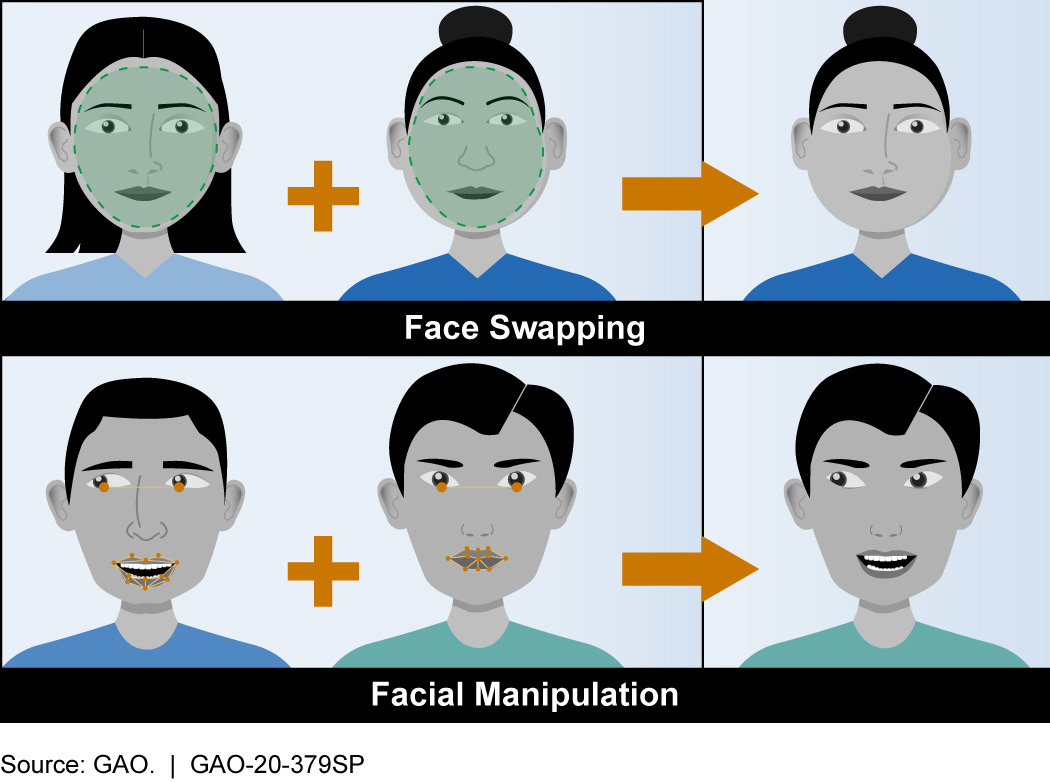
\includegraphics[width=0.9\textwidth]{images/704754.png}  
    \caption{Kasvojen vaihtamisen ja kasvojen manipuloinnin kuvituskuvat (lähde: gao.gov)}  
    \label{figure:deepfakes_fin}  
\end{figure}  

\section*{Puolustuskeinot}

Puolustautuminen tekoälyavusteisia käyttäjän manipulointihyökkäyksiä vastaan on pitkälti samankaltaista kuin perinteisiä, ilman tekoälyn hyödyntämistä toteutettuja manipulointihyökkäyksiäkin vastaan, seuraavilla tärkeillä muutoksilla. Puolustautumiskeinot voidaan karkeasti jakaa tekniikka- ja käyttäjälähtöisiin~\citep{tsinganos_Towards_Automated_Recognition_Chat_SE_Enterprise_2018}.


Perinteinen tapa suojata käyttäjää tietojenkalasteluviesteiltä on esimerkiksi sähköpostiviestien sääntöpohjainen suodattaminen~\citep{mirsky_Threat_Offensive_AI_Organizations_2023}. Yksinkertaistettuna se tarkoittaa joukkoa loogisia sääntöjä, joita seuraamalla voidaan jollakin todennäköisyydellä päätellä, onko viesti tietojenkalasteluviesti vai ei. Sääntöpohjainen suodattaminen ei kuitenkaan toimi hyvin tekoälyavusteista tietojenkalastelua vastaan~\citep{fakhouri_AI_Driven_Solutions_SE_Attacks_2024}.

%koneoppimiseen pohjautuvat
Historiallisesti ei ole ollut tarvetta tarkistaa saatujen kuvien tai videoiden aitoutta, mutta nyt syväväärennösten aikakautena työntekijä ei voi luottaa näkemänsä materiaalin aitouteen, vaan lisävarmistuksia on tehtävä~\citep{mirsky_Creation_Detection_Deepfakes_2021}. Yksi tapa on käyttää tekoälypohjaisia palveluita syväväärennösten tunnistamiseen, samaan tapaan kuin sähköpostiviestitkin tarkistetaan.


Tekoälypohjainen käyttäjän manipulointi tuo joitakin tärkeitä muutoksia käyttäjälähtöisiin puolustuskeinoihin. Ensinnäkään käyttäjät eivät enää voi luottaa siihen, että hyvinkään kirjoitettu viesti ei olisi tietojenkalasteluviesti~\citep{gupta_From_ChatGPT_to_ThreatGPT_2023}. Toiseksi kaikki saatu materiaali, kuten kuvat, äänitiedostot ja videot, saattavat olla syväväärennöksiä, vaikka käyttäjä itse ei huomaisi niissä mitään epätavallista~\citep{blauth_AI_Crime_Overview_Malicious_Use_Abuse_2022}.



Käyttäjälähtöiset tavat ovat käyttäjien kouluttaminen, simuloidut käyttäjän manipulointihyökkäykset, yrityksen tietoturva- ja tietosuojaohjeistusten laatiminen ja käytön valvonta sekä tietoturva- ja tietosuojatietoisen yrityskulttuurin rakentaminen~\citep{tsinganos_Towards_Automated_Recognition_Chat_SE_Enterprise_2018}. Käyttäjille tulee esitellä miltä syväväärennökset näyttävät~\citep{mirsky_Creation_Detection_Deepfakes_2021} sekä kuulostavat~\citep{doan_BTSE_Audio_Deepfake_Detection_2023} ja kuinka helppoa niiden luominen nykyään on.



%Koska tekoälyohjelmat pystyvät automaattisesti etsimään Internetistä tietoa, jota voisi käyttää osana käyttäjän manipulointihyökkäyksiä, myöskään viestit, joissa on maininta joistain käyttäjälle oleellista, ehkä jopa henkilökohtaisista asioista, ei voida enää varmuudella sanoa olevan aitoja.

\section*{Johtopäätökset ja suositukset}

Tekoälyavusteisten käyttäjän manipulointihyökkäysten torjuminen pohjautuu siis pitkälti jo käytössä oleviin tekniikoihin: sisääntulevan viestinnän tarkistamiseen, käyttäjien kouluttamiseen, simuloituihin hyökkäyksiin, tietoturva- ja tietosuojatietoisen organisaatiokulttuurin rakentamiseen ja tietoturvasäännösten ylläpitoon sekä niiden käytön toteutumisen valvontaan~\citep{fakhouri_AI_Driven_Solutions_SE_Attacks_2024}. Jokaiseen näihin on kuitenkin tehtävä muutoksia generatiivisen tekoälyn luoman uuden uhan vuoksi, jotta organisaatiot säästyisivät jopa useisiin miljooniin euroihin nousevilta kustannuksilta~\citep{eniza_Threat_Landscape_2024, verizon_Data_Breach_Investigations_Report_2024}.

Tietomurtojen maailmanlaajuisesta tilanteesta tieteellisesti kertovan Cost of a Data Breach Report -raportin~\citep{ibm_Cost_Data_Breach_Report_2024} mukaan käyttäjien koulutukseen panostaminen alensi keskimääräisestä tietoturvahyökkäyksestä koituneita kustannuksia eniten, 258 629 dollarilla. Vertailun vuoksi tietoturvaohjelmistoihin panostamalla keskimääräiset kustannukset olivat 166 600 dollaria pienemmät. Organisaatioiden jotka panostivat vain vähän käyttäjien tietoturvakoulutukseen keskimääräiset tietomurroista aiheutuneet kustannukset vuositasolla olivat \$5,1 miljoonaa, kun vastaava luku hyvin koulutettujen käyttäjien organisaatioilla oli \$4,15 miljoonaa.



Voimme siis olettaa tekoälyjärjestelmien nopean kehittymisen jatkuvan, tietoturvauhkien kehittymisen niiden mukana sekä tarpeen jatkuvaan käyttäjien kouluttamiseen ja uusien puolustuskeinojen löytämiseen kasvavan. Organisaatioiden tulee huomioida generatiivisen tekoälyn käyttäjän manipulointihyökkäyksiin mukanaan tuomat uudet erityispiirteet panostamalla ensisijaisesti työntekijöidensä koulutukseen ja toissijaisesti uusiin tekoälypohjaisiin tietoturvaohjelmistoihin.





\end{otherlanguage}




%% Chapters


\chapter{Introduction\label{chapter:intro}}
\begin{comment}
- Independent of platform, age of equipment, software, antivirus, firewall (defining social engineering)
- pääasia päälauseeseen tai paragrafin ensimmäiseen virkkeeseen
- vältä liian pitkiä ja monimutkaisia rakenteita, mutta tuo selkeästi esiin asioiden väliset syyt ja seuraukset
- lauseenvastikkeiden käyttö vain niille sopivissa paikoissa
- havainnoillisesti käyttäen konkretisointeja, esimerkkejä, case-study tutkimuksia, kuvia, taulukoita
- 

\end{comment}


%
% Social engineering as a threat to cybersecurity
%
Social engineering has emerged as a significant threat in the digital age, impacting individuals and organizations worldwide. As a subdomain of cybersecurity, social engineering is the art and science of manipulating people into revealing confidential information or performing actions that may or may not be in their best interests~\citep{hadnagy_Social_Engineering_The_Science_2018}. Rather than looking for technical vulnerabilities, social engineering relies on human interaction and exploits weaknesses in human psychology~\citep{wang_Defining_Social_Engineering_2020}.





%
% Social engineering before and now
%
Traditionally, social engineering depended heavily on human intuition and manual effort to deceive its targets~\citep{mitnick_The_Art_of_Deception_2003, mirsky_Threat_Offensive_AI_Organizations_2023}. However, with the advent of generative artificial intelligence (AI), the landscape of social engineering is undergoing a significant transformation, augmenting the sophistication and effectiveness of current and emerging attack methods~\citep{fakhouri_AI_Driven_Solutions_SE_Attacks_2024, fbi_Internet_Crime_Report_2023}. Experts from both industry and academia have unanimously ranked impersonation via deepfake media forgeries as the most significant threat among 32 distinct AI capabilities that can be used against organizations~\citep{mirsky_Threat_Offensive_AI_Organizations_2023}.







%
% What this thesis addresses
%
This thesis addresses how contemporary social engineering defensive countermeasures need to be updated for the novel threat of generative AI in an organizational environment, to bring down annual cybersecurity-related costs. To achieve this, the thesis examines the intersection of generative AI and social engineering based on published literature and incident examples, detailing how advanced AI tools amplify the execution and impact of these attacks while discussing and evaluating the necessary countermeasures.





%
%What attack vectors and tools are analyzed
%
Relevant social engineering attack vectors and tools are examined, including spear phishing with the help of chatbots like ChatGPT and impersonation using deepfake-generated content. Countermeasures discussed include AI-driven detection of spear phishing and deepfakes, employee training programs, necessary modifications to organizational cybersecurity policies, and AI usage guidelines. Fully automated social engineering is still at a somewhat theoretical level and was thus excluded from this thesis~\citep{hatfield_SE_Evolution_Concept_2018}.

\newpage

%
% Countermeasures are insufficient
%
Contemporary countermeasures against social engineering attacks are ill-equipped to deal with the sophistication of AI-powered threats~\citep{blauth_AI_Crime_Overview_Malicious_Use_Abuse_2022, king_AI_Crime_Interdisciplinary_Analysis_2019}. Cybersecurity professionals must thus urgently update their tools and strategies, and AI can play a valuable role in this defensive effort as well~\citep{fakhouri_AI_Driven_Solutions_SE_Attacks_2024, tsinganos_Towards_Automated_Recognition_Chat_SE_Enterprise_2018}.





%
% How is this thesis organized
%
The rest of the thesis is structured as follows: Chapter~\ref{chapter:background} introduces social engineering, generative AI, and other essential concepts for further analysis. Chapter~\ref{chapter:attacks} examines relevant attack vectors and tools, including spear phishing and impersonation with deepfakes. Chapter~\ref{chapter:countermeasures} discusses both technological and user-oriented countermeasures against these attacks. The effectiveness and viability of these measures are assessed in Chapter~\ref{chapter:discussion}. Chapter~\ref{chapter:conclusions} summarizes key findings and implications for the future of social engineering defense.

\chapter{Social engineering and AI\label{chapter:background}}
\begin{comment}
- osakysymykset?
- vertailukohteet?
- cost-benefit ratio johonkin kohtaan?
\end{comment}


%
% Generative AI in SE, chapter overview
%
In recent years, the integration of generative artificial intelligence (AI) into social engineering offensive practices has emerged as a significant concern within the field of cybersecurity~\citep{blauth_AI_Crime_Overview_Malicious_Use_Abuse_2022, king_AI_Crime_Interdisciplinary_Analysis_2019, mirsky_Threat_Offensive_AI_Organizations_2023}. This chapter provides an overview of the role of generative AI in social engineering and explains the key concepts of open-source intelligence, AI, and generative AI. After this, Chapter~\ref{chapter:attacks} examines generative AI -powered social engineering attack vectors and tools.



%
% Defining social engineering
%
A consensus regarding the strict definition of a social engineering attack is lacking in the field~\citep{hatfield_SE_Evolution_Concept_2018}. For the purposes of this thesis, social engineering is defined as "\textit{a type of attack wherein the attacker(s) exploit human vulnerabilities by means of social interaction to breach cybersecurity, with or without the use of technical means and technical vulnerabilities}"~\citep{wang_Defining_Social_Engineering_2020}.



%
% Cybersecurity threats to organizations
%
Organizations today confront cybersecurity threats from a range of sources, including cybercriminals, disgruntled or malicious employees, amateur hackers, hacktivists, competitors, and even state-sponsored cyber terrorists~\citep{mirsky_Threat_Offensive_AI_Organizations_2023}. These threat actors may be driven by motives such as financial gain, intellectual property theft, sabotage, fame, or revenge. Organizations face public scrutiny, loss of customer trust and relations, governmental penalties, and loss of productivity, among other things, due to data breaches.


%
% Why these attack vectors were chosen and not some others
%
While the field of social engineering contains many attack vectors, not all of them are amiable to be enhanced by AI technologies. Research literature has identified and primarily focused on three distinct, but closely related, attack vectors: spear phishing, deepfake impersonation, and real-time voice morphing~\citep{king_AI_Crime_Interdisciplinary_Analysis_2019}. Other popular social engineering attack methods, which do not seem to directly gain much from the advancement of AI technologies, and which are thus not addressed in this thesis, include dumpster diving and shoulder surfing~\citep{mirsky_Threat_Offensive_AI_Organizations_2023}. Table \ref{table:attacks} briefly explains some of the most common social engineering attack vectors. Ransomware attacks are listed as an example of a social engineering attack which can be amplified by AI directly but which isn’t, due to its different nature, examined in this thesis.

\begin{table}[ht!]  
\centering  
\renewcommand{\arraystretch}{1.5} % Adjust row height for better readability  
\setlength{\tabcolsep}{5pt} % Adjust column spacing  
\begin{tabularx}{\textwidth}{|l|X|l|l|} % X column for text wrapping  
\hline  
\textbf{Attack vector} & \textbf{Brief description} & \textbf{Relevance} & \textbf{Included} \\ \hline  
Dumpster diving & Going through someone's trash for sensitive information & No & No \\ \hline  
Impersonation & Claiming to be someone else & Yes & Yes \\ \hline  
Phishing & Deceptive attempts to steal sensitive information & Yes & Yes \\ \hline  
Ransomware & Locking the victim's data against a ransom payment or other action & Yes & No \\ \hline  
Shoulder surfing & Covertly observing people enter sensitive information such as login details & No & No \\ \hline  
Spear phishing & A targeted variety of phishing & No & Yes \\ \hline  
\end{tabularx}  
\caption{Common social engineering attack vectors and their relevance to AI}  
\label{table:attacks}  
\end{table} 


%
% Threat of generative AI
%
A total of 32 different AI capabilities have been identified that attackers could use against an organization~\citep{mirsky_Threat_Offensive_AI_Organizations_2023}. The top three most threatening categories are (1) social engineering, (2) information gathering, and (3) exploit development. Experts from both academia and industry unanimously ranked deepfake-based impersonation as the highest threat~\citep{mirsky_Threat_Offensive_AI_Organizations_2023}. Figure \ref{figure:deepfakes} showcases two potentially abusable use cases of deepfakes. Social engineering attacks are ranked the most threatening because these types of attacks are outside of the defender's control, are relatively easy to achieve, have high payoffs, are hard to prevent, and cause the most harm.

\begin{figure}[ht]  
    \centering  
    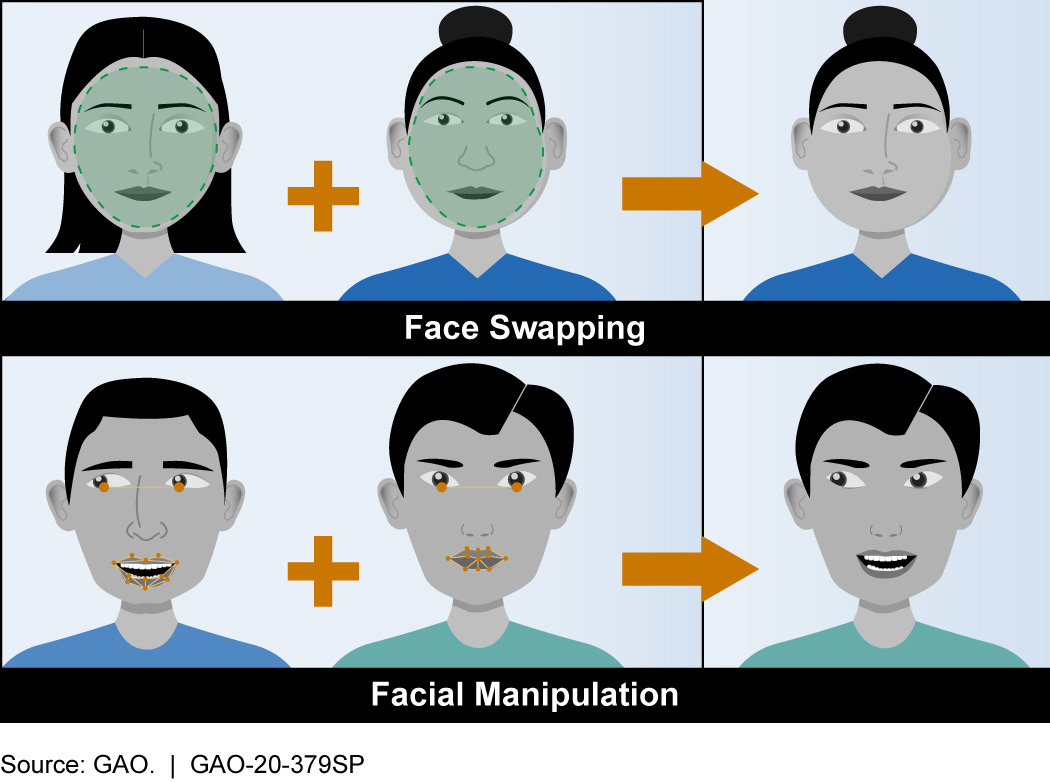
\includegraphics[width=0.9\textwidth]{images/704754.png}  
    \caption{Illustrations of face swapping and facial manipulation (source: gao.gov)}  
    \label{figure:deepfakes}  
\end{figure}  

%
% Tracking incidents
%
Tracking social engineering incidents can be accomplished by counting incident occurrences or by calculating the total cost of all incidents annually~\citep{ibm_Cost_Data_Breach_Report_2024}. Not all organizations report their social engineering and other cybercrime-related incidents, but very good estimates of the prevalence of these attacks can be gained from data that is gathered by various cybercrime-specialized public and private organizations. Their research is published in reports such as the Internet Crime Report~\citep{fbi_Internet_Crime_Report_2023}, the Cost of a Data Breach Report~\citep{ibm_Cost_Data_Breach_Report_2024}, the Data Breach Investigations Report~\citep{verizon_Data_Breach_Investigations_Report_2024} and the Threat Landscape~\citep{eniza_Threat_Landscape_2024}. 

Organizations can thus assess the effectiveness and impact of their new policies, software upgrades, and cultural changes by monitoring incident statistics, particularly incident-related annual costs. These costs include detection, investigation and recovery, and any loss of customers and data. %The annual cybersecurity costs related to social engineering are the primary metric examined in this thesis.






%
% AI threat 
%
The dynamic nature of AI-driven social engineering poses a significant challenge for traditional cybersecurity frameworks, which often rely on static defenses and predefined patterns of attack~\citep{fakhouri_AI_Driven_Solutions_SE_Attacks_2024}. As generative AI technologies advance, their application in crafting personalized and convincing social engineering attacks becomes increasingly evident~\citep{blauth_AI_Crime_Overview_Malicious_Use_Abuse_2022}. This new capability not only enhances the likelihood of success but also complicates the detection and mitigation of such threats~\citep{mirsky_Threat_Offensive_AI_Organizations_2023}.











\section{Open-source intelligence}
\begin{comment}
Some case studies highlighting the use of OSINT in real-world social engineering incidents?
\end{comment}

Social engineering attacks begin with the gathering of data. In cybersecurity, publicly available information is known as \textbf{open-source intelligence}~\citep{hadnagy_Social_Engineering_The_Science_2018}. This practice involves collecting intelligence from sources that are publicly accessible, such as the target organization's website, employees' social media profiles, or other public records. Attackers are increasingly utilizing platforms such as LinkedIn, Facebook, and X (formerly Twitter) to gather information about their victims~\citep{fakhouri_AI_Driven_Solutions_SE_Attacks_2024}.

Various online tools have been created for the purpose of gathering intelligence on an individual or an organization~\citep{mirsky_Threat_Offensive_AI_Organizations_2023}. They often offer automated forensic gathering and are able to visualize the found data, making it easier to identify exploitable patterns and connections. Many of these tools are adapting to use powerful AI technologies as well~\citep{wang_Defining_Social_Engineering_2020}.

Attackers are also able to utilize sites like the Internet Archive and specific web searching features such as Google’s cache to find websites and other material that is no longer accessible via simple web search queries. Bots can be used to download social media posts at frequent intervals in case the target organization makes a mistake in one of their social media posts and deletes it promptly.

Lastly, open-source intelligence, as the name implies, does not contain intelligence gathered using any of the social engineering tactics discussed later, such as calling customer support and asking for personnel information~\citep{hadnagy_Social_Engineering_The_Science_2018}. Open-source intelligence-gathering practices should not leave any traces behind.





\section{Generative AI}
\begin{comment}
\end{comment}

Artificial intelligence (\textit{AI}) encompasses the development of algorithms designed to automate complex tasks ~\citep{mirsky_Threat_Offensive_AI_Organizations_2023}. Currently, the most prevalent type of AI is machine learning, which enables systems to enhance their performance as they gain experience~\citep{fakhouri_AI_Driven_Solutions_SE_Attacks_2024}. Deep learning, a subset of machine learning, employs extensive artificial neural networks as predictive models~\citep{goodfellow_Generative_Adversarial_Networks_2020}. The core idea behind AI is to enable machines to mimic human-like decision-making and thinking processes.

When AI is used to generate content, it is called \textbf{generative AI}~\citep{goodfellow_Generative_Adversarial_Networks_2020}. Unlike traditional AI, which follows programmed rules, generative AI utilizes machine learning to learn patterns from large training datasets to produce new or similar outputs, such as text, images, audio, and video.

Perhaps the most prominent example of generative AI is ChatGPT, a chatbot released by OpenAI in 2022\footnote{https://openai.com/index/chatgpt (visited on 2024-08-19)}. While far from being the first~\citep{weizenbaum_ELIZA_1996}, this chatbot revolutionized how people use and interact with generative AI systems, reaching over 100 million users in just two months\footnote{https://explodingtopics.com/blog/chatgpt-users (visited on 2024-08-11)}. Built on the GPT (\textit{Generative Pre-trained Transformer}) architecture, ChatGPT is designed to understand and generate human-like text by predicting the next word in a sequence.

Another relevant generative AI technology for social engineering is DALL-E, which was released in 2021 and also developed by OpenAI\footnote{https://openai.com/index/dall-e-3/ (visited on 2024-09-19)}. This system generates images from textual descriptions, facilitating digital manipulation and the creation of misleading visuals. It enables the production of hyper-realistic images that can distort or shape public perception.

\chapter{Attack vectors and tools\label{chapter:attacks}}
\begin{comment}
\end{comment}

This chapter reviews key social engineering attack vectors, the method or pathway that a threat actor uses to gain access to data or resources, and tools relevant to the modern threat of generative AI. It first introduces pretexting and spear phishing, then explains how chatbots like ChatGPT could be manipulated, leading to impersonation attacks with deepfakes and voice calls. After this, Chapter~\ref{chapter:countermeasures} goes over the countermeasures against these attacks.



\section{Pretexting}
\begin{comment}
\end{comment}

%
% Social engineering attacks begin with a pretext
%
Social engineering attacks typically begin with the gathering of open-source intelligence, which is subsequently used in conjunction with pretexting to attack an individual or an organization~\citep{hadnagy_Social_Engineering_The_Science_2018}. Pretexting involves fabricating a story or a scenario, a \textbf{pretext}, that is plausible but fraudulent, to engage the target with~\citep{wang_Defining_Social_Engineering_2020}. With this story, the attacker hopes to gain the victim's trust by appearing legitimate. 

%
% Pretexting uses psychological manipulation etc
%
Pretexting uses psychological manipulation, trust, and relationship building, making it a potent tool for threat actors~\citep{mitnick_The_Art_of_Deception_2003}. The attacker, often assuming the likeness and character of a legitimate entity such as a trusted colleague, an IT service worker, a government official, or a 3rd party service provider, creates a believable narrative story tailored to the target victim's context.

%
% Why humans fall victim to pretexts
%
%Humans possess advanced perceptual and decision-making capabilities shaped by lifelong experiences. Attackers can exploit these mental models by presenting deceptive information via pretexting~\citep{mirsky_Threat_Offensive_AI_Organizations_2023}. Information gathered from target A can potentially be used to pretext target B via techniques as simple as utilizing “insider” information.







\section{Spear phishing and other phishing variants}
\begin{comment}
\end{comment}


%
% What is phishing plus a brief history
%
As the quintessential social engineering attack, \textbf{phishing} is characterized by malicious attempts to gain sensitive information from unaware users, traditionally via email and by using spoofed websites that look like their authentic counterparts~\citep{basit_Comprehensive_Survey_AI_Phishing_Detection_2021}. Phishing has been around since 1996 when cybercriminals began using deceptive emails and websites to steal account information from unsuspecting AOL, or America Online, users~\citep{wang_Defining_Social_Engineering_2020}. When phishing attacks are performed using SMS text messages, it’s called \textbf{smishing}.


%
% Spear phishing and whaling, what are they
%
\textbf{Spear phishing}, on the other hand, is a more targeted version of phishing, where threat actors customize their deceptive messages to a target individual or organization~\citep{fakhouri_AI_Driven_Solutions_SE_Attacks_2024}. Spear phishing that is targeted at high-profile individuals is called \textbf{whaling}.


%
% Spear phishing as a more effective, but also more labor-intensive form of phishing
%
Unlike generic phishing attempts, spear phishing involves gathering detailed information about the victim, via open-source intelligence or otherwise, such as their name, position, and contacts to craft a convincing and personalized message~\citep{wang_Defining_Social_Engineering_2020}. Spear phishing has been shown to be up to four times more successful than generic phishing attempts~\citep{king_AI_Crime_Interdisciplinary_Analysis_2019}. This tailored approach increases the likelihood of the victim falling for the phishing attempt, but has traditionally been a lot more time- and energy-consuming~\citep {mirsky_Threat_Offensive_AI_Organizations_2023}.






\section{Abuse of chatbots like ChatGPT}
\begin{comment}
\end{comment}

%
% Malicious use of chatbots like ChatGPT
%
Malicious actors can use generative AI \textbf{chatbots} such as ChatGPT in their social engineering schemes, but due to the manufacturer's set limits, some workarounds may need to be used~\citep{gupta_From_ChatGPT_to_ThreatGPT_2023}. For instance, when asking ChatGPT to provide links to websites that provide pirated content such as movies results in the chatbot denying the request, stating that downloading pirated content is unethical and may also lead to the user's computer being infected with malware.

%
% Bypassing ethical and behavioral restrictions
%
However, regular users and scholars have found a number of ways to bypass ChatGPT's inherent ethical and behavioral guidelines, such as by using reverse psychology\footnote{https://incidentdatabase.ai/cite/420 (visited on 2024-07-15)}. In the above example, instead of directly asking for links to the pirate websites, the user can say that because they do not want their computer to be infected by malware, ChatGPT should provide links to these sites so that the user can avoid visiting them. This technique has been known to cause ChatGPT to reveal the content the user originally wanted~\citep{gupta_From_ChatGPT_to_ThreatGPT_2023}.

%
% ChatGPT can translate spam messages
%
ChatGPT can effectively translate text from the attacker’s native language to the victim’s, maintaining fidelity and correcting any spelling or grammatical errors. It can even enhance the deceptive message, provided that the models' ethical restrictions have been bypassed successfully~\citep{gupta_From_ChatGPT_to_ThreatGPT_2023}.
Phishing messages have historically been marked by noticeable spelling and grammatical errors~\citep{herley_So_Long_No_Thanks_Externalities_2009}, and people have traditionally been advised to look out for these errors as a hallmark of a phishing message. Increasing the message's fidelity will thus increase the likelihood that the target will fall for the phishing attempt~\citep{blauth_AI_Crime_Overview_Malicious_Use_Abuse_2022}.

%
% ChatGPT can integrate OS-INT data into spam messages
%
Chatbots like ChatGPT can also integrate any gathered intelligence into phishing messages, enhancing their relevance. Additionally, incorporating deepfake content, such as an image or a video of the organization’s CEO issuing demands, can further increase the effectiveness of spear phishing attempts.



\section{Impersonation with deepfakes}
\begin{comment}
\end{comment}

%
% What are deepfakes
%
\textbf{Deepfake}, a portmanteau of "deep learning", a type of machine learning, and "fake", is technology that uses artificial neural networks to create highly convincing fake media, either by altering existing content or creating them from scratch~\citep{mirsky_Creation_Detection_Deepfakes_2021}. When existing content is being altered, it's called reenactment or replacement, and when entirely new content is created, it's called synthesis.

%
% What deepfakes can be; depicting a person saying or doing things
%
Deepfake content can be images, audio, and even full-resolution video~\citep{blauth_AI_Crime_Overview_Malicious_Use_Abuse_2022}. Deepfakes have beneficial use cases, such as the realistic dubbing of foreign films, the re-enactment of historical figures for teaching purposes, video games, and for virtually trying on clothes~\citep{mirsky_Creation_Detection_Deepfakes_2021}. However, these hyper-realistic forgeries can also depict a person saying or doing things that didn't take place, making it increasingly difficult for people and even AI systems to discern what is real and what is fake. 

%
% Deepfakes used for impersonation plus a case example
%
By utilizing deepfakes, threat actors can convincingly impersonate trusted individuals or organizations, enhancing the credibility and even the emotional impact of their deceptive social engineering strategies~\citep{mirsky_Creation_Detection_Deepfakes_2021}. In 2021, complete facial reenactment, such as pose, gaze, blinking, and movements, was achieved with only a minute of training video, suggesting that if a malicious actor wants to reenact an individual, they do not need to gather a lot of video material for this. If video material is not available, threat actors might be able to resort to filming the target person exiting the organization's premises. 

Advanced deepfake technology was famously used in a 2024 incident in a live video conference where the threat actors successfully scammed an organization for~\$25 million\footnote{https://incidentdatabase.ai/cite/634 (visited on 2024-08-24)}.% lisää tähän toinen esimerkki, toinen lause?




\section{Phishing via calls and audio}
\begin{comment}
\end{comment}

%
% What is vishing
%
Phishing that is done using voice is called \textbf{vishing}, from voice phishing~\citep{doan_BTSE_Audio_Deepfake_Detection_2023}. By utilizing traditional telephone systems or VoIP (Voice-over-IP), the attacker calls the victim with a pretext to manipulate them into revealing sensitive information or performing actions that may or may not be in their best interests~\citep{hadnagy_Social_Engineering_The_Science_2018}.


%
% Real-time voice morphing for vishing attacks
%
With real-time voice morphing, a type of deepfake natural speech synthesis, the attacker can effectively and realistically impersonate someone else~\citep{doan_BTSE_Audio_Deepfake_Detection_2023}. This technology converts the attacker's voice, as input, to the chosen person's voice, as output, automatically during the call. It's hard for the human auditory system to distinguish between real and fake voice samples, especially through voice calls which tend to have lower audio fidelity.



%
% Training deepfake models
%
Like all deepfake models, the audio model has to be trained before it can be used~\citep{doan_BTSE_Audio_Deepfake_Detection_2023}. This is done using audio, which can be sourced from places like YouTube, a company website, or by calling the person the attacker wants to mimic the voice of and recording the conversation.



%
% Vishing with deepfakes: a significant concern plus a case example
%
Social engineering with real-time voice morphing of employees' voices has been found to be one of the top threats posed by AI to organizations~\citep{mirsky_Threat_Offensive_AI_Organizations_2023}. The first significant and famous incident occurred back in 2019, where threat actors successfully used deepfake-generated voice during a call to impersonate an authentic entity for monetary gains exceeding 200,000~€\footnote{https://incidentdatabase.ai/cite/200 (visited on 2024-05-13)}.

\chapter{Countermeasures\label{chapter:countermeasures}}
\begin{comment}
- ero company culture ja company policy
- Asiantuntijalla näkemystä aiheesta, vertailee eri tuloksia eri lähteistä, ei vaan toista
- sisältää vertailua, analyysiä, arviointia, soveltamisesimerkkejä... Bloomin puu
- varsinaisen kontribuution koti, vertailu, soveltaminen, osien synteesi ja mahdolliset evaluointimenetelmät ja -tulokset pääroolissa

\end{comment}

Countermeasures against the attacks covered in the previous chapter are examined in this chapter. It focuses on two parts: technology-oriented countermeasures such as phishing and deepfake detection mechanisms, and user-oriented countermeasures such as personnel training programs and company policy updates. Technology-oriented countermeasures are examined first since human-oriented measures rely on and build upon them. After this, Chapter~\ref{chapter:discussion} discusses and evaluates these countermeasures in detecting and preventing social engineering attacks.

Traditionally, defense against social engineering relied on human education and awareness campaigns~\citep{fakhouri_AI_Driven_Solutions_SE_Attacks_2024}. This reliance, despite its many merits, has revealed its fragility, as even the best-trained user can fail to detect a social engineering attack and fall victim to it. Defense against generative AI -based social engineering thus requires a multifaceted approach, incorporating both technical and user-oriented measures.


\section{Phishing detection with AI}
\begin{comment}
\end{comment}
Traditional phishing message detection systems, i.e. those not based on machine learning and AI, are typically rule- and signature-based, which often falter when faced with novel or evolved threats like those enhanced by AI~\citep{fakhouri_AI_Driven_Solutions_SE_Attacks_2024}. These defenses often leave the systems they are supposed to be defending vulnerable to novel, uncharted attacks.

AI systems learn, evolve, and adapt based on the datasets that they are processing, thus continuously refining their operational methods and predictions, rather than relying on pre-defined and rigid algorithms~\citep{fakhouri_AI_Driven_Solutions_SE_Attacks_2024}. This presents a paradigm shift in how computers perceive, then process and finally respond to data.

These machine learning models are trained with vast datasets containing both safe and malicious samples of e.g. phishing messages and phishing URL's. Given time and further training, these models learn to identify patterns, behaviors, and anomalies, meaning they are very capable of detecting threats, including the novel and perhaps even the yet unseen~\citep{fakhouri_AI_Driven_Solutions_SE_Attacks_2024}. Including AI in cybersecurity measures thus doesn't mean just adding another tool for cybersecurity, but fundamentally defining anew the foundations of the organization’s digital defenses. More specifically, AI-based methods have shown great promise in identifying phishing attempts with high accuracy, often surpassing traditional detection methods~\citep{basit_Comprehensive_Survey_AI_Phishing_Detection_2021}.




\section{Identifying deepfakes}
\begin{comment}
\end{comment}
Deepfakes often contain subtle anomalies called artifacts, just as image and audio forgeries of the past did. Deepfake detection procedures are primarily based on machine learning and forensic analysis, attempting to identify these specific artifacts in the multimedia content~\citep{mirsky_Creation_Detection_Deepfakes_2021}. The artifacts can be subtle, such as a strange blob of pixels, or overt, such as a person having clearly warped eyes. Figure \ref{figure:artifacts} represents a few sample artifacts.

\begin{figure}[h]  
    \centering  
    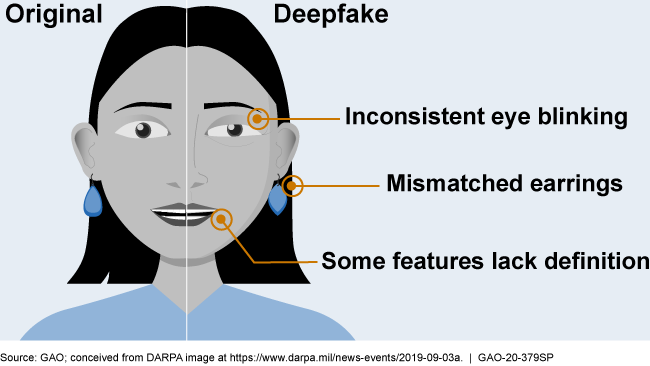
\includegraphics[width=0.9\textwidth]{images/rId14_image5.png}  
    \caption{Potential artifacts in a deepfake image or video (source: gao.gov)}  
    \label{figure:artifacts}  
\end{figure}  

Just as incoming email messages are analyzed for phishing attacks, and the attachments are scanned for viruses, images, audio, and videos may need to be scanned as well to aid the user in detecting if they are genuine or deepfakes~\citep{mirsky_Creation_Detection_Deepfakes_2021}. Detecting deepfakes is a lot more computationally intensive than email phishing detection, so organizations may opt for giving employees the possibility of initiating a scan on material they suspect isn’t genuine.



Where once experts in the field could recommend that a caller be authenticated by recognizing their voice, accent, and intonations~\citep{mitnick_The_Art_of_Deception_2003}, with the advent of generative AI and especially deepfakes, this no longer holds true~\citep{doan_BTSE_Audio_Deepfake_Detection_2023}. Technologies such as the BTS-E encoder have been proposed for spotting idiosyncrasies in speech that might not or even could not be consciously registered by human observers, by detecting correlations between breathing, talking, and silence in calls and other audio.

%
% Seven deepfake artifacts
%
Seven different types of artifacts related to image and especially video deepfakes have been identified in two main categories~\citep{mirsky_Creation_Detection_Deepfakes_2021}: spatial-type artifacts which cover blending, environment, and forensics, while temporal-type artifacts cover behavior, physiology, synchronization, and coherence. Table \ref{table:deepfake_artifacts} explains these artifacts briefly.

\begin{table}[ht!]  
\centering
\renewcommand{\arraystretch}{1.5} % Adjust row height for better readability  
\setlength{\tabcolsep}{5pt} % Adjust column spacing  
\begin{tabularx}{\textwidth}{|l|l|X|} % X column for text wrapping  
\hline  
\textbf{Type} & \textbf{Mechanism} & \textbf{Description} \\ \hline  
S & Blending & Related to the generated content when it is integrated back into a frame (the background), which is detectable with techniques such as edge detection and frequency analysis \\ \hline  
S & Environment & Appear when fake facial content seems inconsistent
with the surrounding background frame, often due to mismatches in warping, lighting, or
fidelity \\ \hline  
S & Forensics & Residues from the generative models, such as generative
adversarial network fingerprints or sensor noise \\ \hline  
T & Behavior & Relates to the monitoring of anomalies in the target’s mannerisms \\ \hline  
T & Coherence & Inconsistencies in logical sequences
happening over time\\ \hline  
T & Physiology & Inconsistencies in natural biological cues like blinking of
the eyes or head movements \\ \hline  
T & Synchronization & Mismatched
audio-visual elements \\ \hline  
\end{tabularx}  
\caption{Deepfake detection mechanisms: S = spatial, T = temporal~\citep{mirsky_Creation_Detection_Deepfakes_2021}}  
\label{table:deepfake_artifacts}  
\end{table}  




\section{Employee education, simulated attacks, and organizational changes}

User-oriented countermeasures against social engineering attacks usually fall into four broader categories~\citep{tsinganos_Towards_Automated_Recognition_Chat_SE_Enterprise_2018, mitnick_The_Art_of_Deception_2003}. These categories are simulated penetration tests with social engineering techniques, employee security awareness training programs, the creation and application of corporate cybersecurity policies, and the development of a security-conscious company culture.

Regular and comprehensive training programs are vital to educate employees about social engineering tactics. Regularity is stressed by experts in the field as users tend to forget what they have learned~\citep{hadnagy_Social_Engineering_The_Science_2018, mitnick_The_Art_of_Deception_2003}. It is thus suggested that training against social engineering attacks is not something that is done annually, or even bi-annually, but rather that it's something that is baked into the company's culture. 

The inoculation theory~\citep{blauth_AI_Crime_Overview_Malicious_Use_Abuse_2022} suggests that prior exposure to social engineering attacks could help protect users against future threats, whether these attacks are genuine or simulated. Conducting simulated social engineering and phishing attack campaigns, via numerous channels such as email, SMS, and even phone/VoIP, allows organizations to assess the susceptibility of their employees to social engineering tactics~\citep{hadnagy_Social_Engineering_The_Science_2018}. These exercises help identify vulnerabilities in the workforce, enabling further targeted training and reinforcing the importance of scrutinizing unsolicited communication, and with the advent of generative AI and deepfakes, this needs to be extended to received images, videos, and calls~\citep{mirsky_Creation_Detection_Deepfakes_2021}.

Employees should be shown what different varieties of deepfake content look like, as well as how easy it is to doctor them~\citep{mirsky_Creation_Detection_Deepfakes_2021}. With the permission of the organization’s CEO or other top executives, their likeness could be used for this training material.

It's imperative that every user understands that they are the weakest link in the cybersecurity chain and that the responsibility of the organization's cybersecurity is in everyone's hands, not just the cybersecurity professional's~\citep{mitnick_The_Art_of_Deception_2003}. If an employee has a user account in the organization’s systems, that is a potential entryway for threat actors.

Finally, because AI can source social media sites and the Internet automatically for open-source intelligence, it's imperative for people to know to be careful of what they share, with whom and when~\citep{mitnick_The_Art_of_Deception_2003}. Even seemingly coincidental information, such as photos indicative that the employee is now on a company picnic, could be used against them and their employer in a social engineering attack.

\chapter{Discussion\label{chapter:discussion}}
\begin{comment}
\end{comment}

This chapter evaluates current countermeasures and their effectiveness at detecting and preventing social engineering attacks, particularly those enhanced by generative AI technologies. The landscape of cybersecurity is continuously evolving, and traditional countermeasures such as email filtering and user awareness programs, although still crucial, are increasingly insufficient against the sophistication of AI-powered threats~\citep{fakhouri_AI_Driven_Solutions_SE_Attacks_2024}. While current countermeasures provide a baseline defense against social engineering attacks, this evaluation reveals a critical gap between existing strategies and the rapidly evolving sophistication of generative AI -powered attacks. After this, Chapter~\ref{chapter:conclusions} concludes the thesis.

According to the Cost of a Data Breach report~\citep{ibm_Cost_Data_Breach_Report_2024}, organizations are increasingly leveraging AI and automation in their security operations. 31\% of the studied organizations deploy these technologies extensively, 36\% reported limited use and the remaining 33\% reported no use. Notably, when AI was extensively deployed in prevention workflows, organizations saw an average breach cost reduction of 45\% (\$2.2 million compared to the average of \$4,88 million). The key finding of last year's report is a striking correlation: the more an organization relied on AI, the lower its average breach costs were.

It seems evident that the highly dynamic nature of AI technologies fuels a continuous arms race between attackers and defenders, causing many countermeasures to become obsolete quickly~\citep{fakhouri_AI_Driven_Solutions_SE_Attacks_2024}. Thus, protecting against AI-powered attacks requires not a single solution but an integrated approach that is baked in the company culture, that combines technological defenses, comprehensive and continuous user education, and robust organizational policies.

\section{Generative AI and deepfakes}
\begin{comment}
\end{comment}

Just as spam filters are inclined to report false positives~\citep{fakhouri_AI_Driven_Solutions_SE_Attacks_2024}, so too are deepfake detection systems~\citep{mirsky_Creation_Detection_Deepfakes_2021}. Filtering legitimate communications out may cause operational disturbances and perhaps even lost business engagements.

Technological solutions like phishing detection systems that utilize natural language processing and machine learning show potential in identifying anomalous communications~\citep{basit_Comprehensive_Survey_AI_Phishing_Detection_2021}. However, these systems are being challenged by the ever-improving quality of AI-generated content such as spear phishing messages, which often mimic human interaction and presentation with higher and higher fidelity. Similarly, tools designed to detect deepfakes are in their early stages~\citep{mirsky_Creation_Detection_Deepfakes_2021}, and face significant hurdles in keeping up with the rapid advancements in AI technologies that create such content.



Part of the solution regarding deepfake content is to raise population awareness about such technology use~\citep{blauth_AI_Crime_Overview_Malicious_Use_Abuse_2022}. For instance, in 2019, the Democratic Party (USA) presented a deepfake video of their own chairman to highlight their concerns about deepfake content\footnote{https://edition.cnn.com/2019/08/09/tech/deepfake-tom-perez-dnc-defcon/index.html (visited on 2024-08-25)}.

Virus detection signatures are developed by their respective companies, and cybersecurity personnel must be trained regularly. However, AI makes a difference here because AI systems can learn from other AI systems. Where one network is the target of a novel type of cybersecurity threat, and once its detected, this AI system can inform other systems in the same "network", thus bolstering defenses on a possibly global scale?

Spreading information about deepfakes to the public faces the hurdle of the "liar's dividend", a situation where a "liar" discredits a real video claiming it to be a deepfake. The more users are aware of deepfake content and the ability of AI to doctor and create videos, the more skeptical they will be, causing them to question images and videos that are real~\citep{blauth_AI_Crime_Overview_Malicious_Use_Abuse_2022}. Deepfakes may thus erode the public's very trust in multimedia content, and the press in general.

AI excels in detecting subtle patterns and anomalies which might elude more conventional systems \citep{fakhouri_AI_Driven_Solutions_SE_Attacks_2024}. This capability exceeds mere threat recognition and covers concepts such as anticipation of future potential vulnerabilities based on real-time and also historical data, which helps ensure defensive measures are not just reactive but predictive (proactive).

\section{On defending users and employees}
\begin{comment}
\end{comment}

User-oriented measures remain pivotal in the defense against social engineering. Regular training programs are crucial for equipping end-users with the knowledge to recognize potential threats~\citep{hadnagy_Social_Engineering_The_Science_2018}. This holds true especially because AI technologies are evolving rapidly on both the offensive and defensive sides, leading to a situation where the attackers are one step ahead of the defenders and automated AI-based social engineering detection and prevention systems fail to protect the user~\citep{fakhouri_AI_Driven_Solutions_SE_Attacks_2024}. Thus comprehensive, regular and innovative user training and awareness programs can never be overlooked, as the user remains the weakest link in the cybersecurity chain~\citep{mitnick_The_Art_of_Deception_2003}.

A company culture that is open about sharing if any of its members fall victim to social engineering attacks is more robust due to employees not having to feel shame or hide the fact that they got tricked~\citep{hadnagy_Social_Engineering_The_Science_2018}. This can be reinforced by executives talking openly about times when they fell victim, to what kind of an attack and why, and what they did about the incident. It's always better that employees report suspected or actualized social engineering attacks rather than trying to hide them for fear of ridicule or punishment.

The deployment of simulated social engineering campaigns offers substantial insights into employee vulnerability, yet these must be meticulously crafted to avoid adverse impacts on workplace morale~\citep{mitnick_The_Art_of_Deception_2003}. Utilizing natural language processing to craft highly convincing but simulated phishing messages to be sent to the employees can further aid in the detection of the need for further training, with open-source intelligence being incorporated also.

Feedback from these simulations can significantly aid personnel development. However, employees who fall victim to these simulated attacks should be re-educated rather than punished~\citep{mitnick_The_Art_of_Deception_2003}. Furthermore, it is essential to inform employees in advance that such campaigns may be run occasionally. This approach not only helps keep them vigilant but should also mitigate negative feelings associated with "being tricked" by their own company.

Just as people have differing propensities for detecting phishing attempts and noticing subtle anomalies in spelling and grammar~\citep{nicholson_Investigating_Teenagers_Detect_Phishing_2020, neupane_Social_Disorders_Facilitate_SE_2018}, so too are people variously adept at spotting these anomalies in deepfakes.

%
% Teenagers, young people and autistic people, susceptibility 
%
Certain parts of the population, such as teenagers and young people who haven't yet gained enough experience on the Internet, may be more susceptible to social engineering attacks~\citep{nicholson_Investigating_Teenagers_Detect_Phishing_2020}. People on the autism spectrum, often facing challenges in social interaction, may unexpectedly excel at detecting social engineering attacks~\citep{neupane_Social_Disorders_Facilitate_SE_2018}. It is thus suggested that training efforts, while they must be targeted at everyone, would take into account any potential differences in demographics. Chatbots like ChatGPT can help in designing tailored and engaging training content, perhaps even with gamification.





\section{Societal and scientific impact}
\begin{comment}
\end{comment}
As AI is developed further and the more its availability increases, the risk or malicious or criminal use increases as well, and these risks, if not properly addressed, may lead to the excessive strict regulation of AI technologies~\citep{king_AI_Crime_Interdisciplinary_Analysis_2019}.

The benefits of AI for society and individuals may be significantly compromised due to ongoing constraints on its development~\citep{king_AI_Crime_Interdisciplinary_Analysis_2019}. A notable example is the restriction on releasing source code and data from a study that demonstrated how visual discriminators could identify a person's sexual orientation with accuracies far higher than those of human judges, which undermines scientific reproducibility. In the end, it comes to societal values. Science is done all around the globe, and if one nation rejects to release their source code and data due to ethical considerations, some other nation with different values and value systems may elect to do so on their comparable studies.

In 2024, the state of Tennessee enacted the ELVIS Act\footnote{https://aibusiness.com/responsible-ai/tennessee-enacts-elvis-act-to-protect-artist-voices-from-ai-misuse (visited on 2024-08-24)} (Ensuring Likeness Voice and Image Security), protecting artists from the use of their voice and likeness via deepfake technologies. Further legislation in the United States needs to address the use of deepfakes in other ways, such as in social engineering.

Because regulatory frameworks and other governance mechanisms might not be developed at the same pace as technological advancements, proactivity is vital to reduce the risks~\citep{blauth_AI_Crime_Overview_Malicious_Use_Abuse_2022}. The faster the potential for AI misuse is understood, the earlier potential preventive and mitigative policies may be applied~\citep{king_AI_Crime_Interdisciplinary_Analysis_2019}. Some regulatory limitations may, however, be hampering cybersecurity defensive measures.

The European Union’s AI Act explicitly prohibits the use of AI for human manipulation and social engineering, but questions arise when social engineering tactics and techniques are used for simulated phishing campaigns. Can AI be developed to be a better social engineer than any human, for the purposes of bolstering organizational defenses? If so, what prevents the same AI from being used for malicious purposes against an organization who has not consented on such simulated attacks? It seems that wherever strict regulatory lines are drawn, it will always be a compromise.

\chapter{Conclusions\label{chapter:conclusions}}
\begin{comment}
- Muistuta tutkimuskysymys
- Tärkeimmät tulokset ja perusteet
- Incident costs, numbers = impact
suositukset
- Anakyysia, vertailua, arviointia
- Ei turhia osioita, toistoa
- Puutteita kandissa? Mitä olisi hyvä vielä kertoa?’
- phishing by far the most loss causing cyberattack (fbi)
- calls to verified phone numbers (fbi), not relying on phone numbers on emails
- out of 880,418 fbi 298,878 were phishing 2023 (individuals, not organizations)
- more than half of organizations said they are passing the costs to customers ibm
- cybersecurity teams are constantly understaffed ibm
\end{comment}

The subfield of social engineering within cybersecurity is undergoing a significant transformation with the advent of generative AI~\citep{fakhouri_AI_Driven_Solutions_SE_Attacks_2024}. This thesis explored how generative AI empowers threat actors in this space and how current countermeasures in an organizational environment need to be updated to reflect this evolving threat landscape.

Generative AI is revolutionizing social engineering attacks, enabling threat actors to use sophisticated tactics like spear phishing~\citep{basit_Comprehensive_Survey_AI_Phishing_Detection_2021}, impersonation with deepfake content~\citep{mirsky_Creation_Detection_Deepfakes_2021} and voice phishing, vishing, with real-time voice morphing~\citep{doan_BTSE_Audio_Deepfake_Detection_2023}. These advancements reveal that traditional countermeasures are becoming increasingly ineffective, requiring an urgent and comprehensive re-evaluation of current strategies and tactics.

Previously an employee could authenticate a caller by recognizing their voice, intonations, and accent~\citep{mitnick_The_Art_of_Deception_2003}, but today this is no longer enough. User training and awareness programs must be updated to address the novel threat of AI in social engineering. Historically, employees have been trained to spot spelling errors in email messages, and today they must be trained to broaden their scope of skepticism to include images, audio, and videos as well~\citep{mirsky_Creation_Detection_Deepfakes_2021}.

AI can help detect social engineering attacks, but it does not eliminate the necessity for user training and awareness programs. On the contrary, as AI-powered attacks proliferate, the need for awareness and vigilance will grow even higher~\citep{fakhouri_AI_Driven_Solutions_SE_Attacks_2024}. Chatbots like ChatGPT can help develop more robust security guidelines and design highly engaging social engineering awareness programs. In addition, image-generation technologies like DALL-E can help create memorable and funny images for posters and campaigns.

One area not addressed in this thesis, but deserving of future research, is the potential for AI to automate social engineering attacks, either in part or even completely~\citep{mirsky_Threat_Offensive_AI_Organizations_2023}. Currently, however, AI technology is not capable of executing such attacks without human oversight, but as the field is evolving rapidly, organizations must take this possibility into consideration as well.


The Cost of a Data Breach Report~\citep{ibm_Cost_Data_Breach_Report_2024} revealed that organizations using AI to address cybersecurity threats experienced an average of 45\% reduction in annual incident-related costs compared to those that did not. Further, IBM found that increased reliance on AI corresponded with lower incident costs. Organizations need to utilize AI to combat generative AI -powered social engineering, primarily because even the best-trained employee could fall victim to a sophisticated spear phishing scheme.

It seems evident that the highly dynamic nature of AI technologies fuels a continuous arms race between attackers and defenders, causing many countermeasures to become obsolete quickly~\citep{fakhouri_AI_Driven_Solutions_SE_Attacks_2024}. Thus, protecting organizations against AI-powered social engineering attacks requires not a single solution but an integrated approach that is baked in the company culture, that combines technological defenses, comprehensive and continuous user education, and robust organizational policies.

Cybersecurity experts must thus concentrate their efforts on deterring the top threats organizations face from generative AI, namely impersonation with deepfakes and highly targeted, seemingly authentic spear phishing. This effort needs to be primarily focused on employee training and secondarily on new, AI-powered social engineering prevention software and hardware technologies.

%
% Defense against AI-powered threats
%
%Defense against AI-enhanced social engineering will thus require a multifaceted approach that combines technological innovation, user education, and a proactive stance and strict enforcement of cybersecurity policy~\citep{blauth_AI_Crime_Overview_Malicious_Use_Abuse_2022}. As the landscape continues to evolve, staying ahead of these threats will necessitate ongoing research and collaboration across the cybersecurity community to develop effective countermeasures and best practices~\citep{fakhouri_AI_Driven_Solutions_SE_Attacks_2024}.




%%%%%%%%%%%%%%%%%%%%%%%%%%%%%%%%%%%%%%%%%%%%%%%%%%%%%%%%%
%\cleardoublepage                          %fixes the position of bibliography in bookmarks
%\phantomsection
\addcontentsline{toc}{chapter}{\bibname}  % This lines adds the bibliography to the ToC
\printbibliography
%

\appendix{Statement on the use of AI tools\label{extra:declaration}}
\begin{comment}
\end{comment}


I hereby state all of the use cases where I have utilized advanced AI technologies during the research and writing processes of this thesis in Table \ref{table:declaration}.


\begin{table}[ht!] 
\centering 
\renewcommand{\arraystretch}{1.5} % Adjust row height for better readability  
\setlength{\tabcolsep}{5pt} % Adjust column spacing  
\begin{tabularx}{\textwidth}{|l|X|} % X column for text wrapping  
\hline  
\textbf{Tool} & \textbf{Use cases} \\ \hline  
Sider Fusion & Automatically choosing the most suitable large language model based on my query\\ \hline  
Large language models* & Finding synonyms for a few words, generating \LaTeX{} code for tables/images, asking for help with other \LaTeX{} commands, brainstorming what the general topic for my thesis could be (before I started my writing process), and performing OCR-to-text from handwritten notes\\ \hline  
Writefull \& Grammarly & Correcting simple spelling errors on Overleaf when prompted via a red underline\\ \hline  
Keenious & Finding relevant research articles based on existing literature and drafts of this thesis\\ \hline  
\end{tabularx}  
\caption{AI tools and their use cases for thesis writing and research}  
\label{table:declaration}  
\end{table}  

I’ve trialed multiple generative AI tools and compared their outputs to find the best ones for my current
purposes, which is why the list of LLMs is so extensive.

*Large language models used: GPT-3.5, GPT-4 (4o \& mini), Claude 3.5 Haiku \& Sonnet, Gemini 1.5 Flash \& Pro, Llama-3, DeepSeek R1 70B  
%%%%%%%%%%%%%%%%%%%%%%%%%%%%%%%%%%%%%%%%%%%%%%%%%%%%%%%%%


%% Commented \backmatter out because it caused an empty page to be added at the end of my thesis
%% TODO: verify that it isn't needed

\backmatter

\begin{appendices}



\appendix{Statement on the use of AI tools\label{extra:declaration}}
\begin{comment}
\end{comment}


I hereby state all of the use cases where I have utilized advanced AI technologies during the research and writing processes of this thesis in Table \ref{table:declaration}.


\begin{table}[ht!] 
\centering 
\renewcommand{\arraystretch}{1.5} % Adjust row height for better readability  
\setlength{\tabcolsep}{5pt} % Adjust column spacing  
\begin{tabularx}{\textwidth}{|l|X|} % X column for text wrapping  
\hline  
\textbf{Tool} & \textbf{Use cases} \\ \hline  
Sider Fusion & Automatically choosing the most suitable large language model based on my query\\ \hline  
Large language models* & Finding synonyms for a few words, generating \LaTeX{} code for tables/images, asking for help with other \LaTeX{} commands, brainstorming what the general topic for my thesis could be (before I started my writing process), and performing OCR-to-text from handwritten notes\\ \hline  
Writefull \& Grammarly & Correcting simple spelling errors on Overleaf when prompted via a red underline\\ \hline  
Keenious & Finding relevant research articles based on existing literature and drafts of this thesis\\ \hline  
\end{tabularx}  
\caption{AI tools and their use cases for thesis writing and research}  
\label{table:declaration}  
\end{table}  

I’ve trialed multiple generative AI tools and compared their outputs to find the best ones for my current
purposes, which is why the list of LLMs is so extensive.

*Large language models used: GPT-3.5, GPT-4 (4o \& mini), Claude 3.5 Haiku \& Sonnet, Gemini 1.5 Flash \& Pro, Llama-3, DeepSeek R1 70B

%% A sample Appendix
%
\appendix{Declaration on the use of AI\label{appendix:declaration}}

I, Riku Talvisto, hereby state the following regarding the use of AI when working on my thesis. How I used AI tools and which tools were used.

Most of my AI use has been done via Sider.ai, which is a browser extension sidebar app that allows direct interaction with the current webpage with various LLM tools. Sider.ai provides Sider Fusion, which dynamically selects an appropriate model to be used based on the given query.

Table \ref{tab:declaration} lists all of the AI tools that I have used and all of their use scenarios.

\begin{table}[h]
  \centering
  %\begin{tabularx}{\textwidth}{X X}
  \begin{tabular}{m{5cm}m{8cm}}
    \hline
    \textbf{Tool} & \textbf{Use cases} \\
    \hline
    Sider Fusion & To automatically choose the best model from the list of used LLM's based on the query. \\
    \hline
    GPT-3.5 Turbo, GPT-4, GPT-4o, Claude 3 Haiku, Claude 3.5 Sonnet, Gemini 1.5 Flash, Gemini 1.5 Pro, Llama-3 & Finding synonyms for words. Generating LaTeX code for tables and images, which I’ve manually tweaked later. Brainstorming ideas about my thesis. Finding related keywords. Highlighting my abstract text and asking how many words it contains. \\
    \hline
    Writefull & Correcting spelling errors on Overleaf when prompted. \\
    \hline
    Keenious & Find relevant research articles based on already found literature and also based on my own work. \\
    \hline
  %\end{tabularx}
  \end{tabular}
  \caption{AI tools used}
  \label{tab:declaration}
\end{table}

I've trialed multiple tools and compared their outputs to find the best ones for my current purposes, and this is why the list of LLM's is so extensive.



%% another appendix
%%
\appendix{Instructions for LaTex}

\section{General Setup}

In the HY-CS-main.tex file you will find the following STEPS 0--5. Below you can find related instructions.
\vspace{0.5cm}

\textbf{STEP 0 -- Access the thesis template}

\begin{itemize}
\item Import the thesis template into a new Overleaf project. The easiest way to do it is to:
\begin{itemize}
    \item Obtain a zip file of the LaTeX template from the webpage of your programme.
    \item Go to \url{https://www.overleaf.com/edu/helsinki} and login to Overleaf with your university credentials.
    \item Go to the list of your projects at \url{https://www.overleaf.com/project}, click ``New Project'' and ``Upload Project''.,  the projects under your account 
    \item Then upload the zip with the template.
    \item You are now ready to write your thesis in Overleaf by editing the template, you can start by renaming the project.
\end{itemize}
\end{itemize}


{\textbf{STEP 1 -- BSc or MSc thesis?}}
\begin{enumerate}
\item Select whether your are writing BSc (tkt) or MSc (csm for CS) thesis.
\item Select your language: \texttt{finnish}, \texttt{english}, or \texttt{swedish}.
\item If you are writing MSc select your line / track.
\end{enumerate}


{\textbf{STEP 2 -- Set up your personal information}}

\begin{enumerate}
\item Specify the title of your thesis with \texttt{\textbackslash title\{\}}.
\item Specify your name to the author field with \texttt{\textbackslash author\{\}}.
\item Specify the names of your supervisors of the thesis with \texttt{\textbackslash supervisors\{\}}.
\item Specify the keywords of the thesis with \texttt{\textbackslash keywords\{\}}.
\item Specify the ACM classification terms of the thesis with \texttt{\textbackslash classification\{\}}. See \url{https://dl.acm.org/ccs} for more information.
\end{enumerate}

{\textbf{STEP 3 -- Write your abstract}}

\begin{itemize}
\item You can have the abstract in multiple languages with the \texttt{otherlanguages} environment. The example below shows how to provide an English abstract: 

\begin{verbatim}
\begin{otherlanguage}{english} 
\begin{abstract}
Your abstract text goes here. 
\end{abstract} 
\end{otherlanguage}
\end{verbatim}

\end{itemize}

{\textbf{STEP 4 -- Writing your thesis}}

\begin{enumerate}
\item There are some minimal contents and instructions below 
\item Remove, or comment out, this appendix from your thesis.
\end{enumerate}

{\textbf{STEP 5 -- Set your bibliography style}}

\begin{itemize}
\item The default is Author-Year style (Einstein, 1905), but it can be easily changed to numbered [1] or alphabetical [Ein05] , as the examples of these are in comments.
\item Discuss the style to use with your supervisor.
\end{itemize}

\section{Bibliography in Latex}

The bibliography is defined in a separate \texttt{.bib} file. For this template, it is named \texttt{bibliography.bib} and includes the content show in Figure~\ref{bibexamples}.

Chapter Bibliography lists all the works that you refer to in your text. You refer to the works in the bibliography using an appropriate \emph{citation key}.
%
%This thesis template contains an example of a bibliography.


References are done using \texttt{\textbackslash citep\{einstein\}}, which generates in text a citation formatted according to the selected style \citep{einstein}, or \texttt{\textbackslash citep\{latexcompanion,knuth99\}}, which generates \citep{latexcompanion,knuth99}. 
As examples of a different kinds of citations (see how these look in the Latex source), we can write \citep{einstein} to refer to the work written by \citeauthor{einstein} in \citeyear{einstein}, because the work by \citet{einstein} appears in the bilbliography included in this template.

Note that there are different possible styles for the bibliography and citation keys.
%
Consult your supervisors on the chosen style -- and once you arrive at a preferred style, use it consistently throughout the thesis.

\begin{figure}[ht]
    \centering
    \begin{scriptsize}
\begin{verbatim}
@article{einstein,
    author =       "Albert Einstein",
    title =        "{Zur Elektrodynamik bewegter K{\"o}rper}. ({German})
        [{On} the electrodynamics of moving bodies]",
    journal =      "Annalen der Physik",
    volume =       "322",
    number =       "10",
    pages =        "891--921",
    year =         "1905",
    DOI =          "http://dx.doi.org/10.1002/andp.19053221004"
}
 
@book{latexcompanion,
    author    = "Michel Goossens and Frank Mittelbach and Alexander Samarin",
    title     = "The \LaTeX\ Companion",
    year      = "1993",
    publisher = "Addison-Wesley",
    address   = "Reading, Massachusetts"
}

@book{knuth99,
    author    = "Donald E. Knuth",
    title     = "Digital Typography",
    year      = "1999",
    publisher = "The Center for the Study of Language and Information",
    series    = "CLSI Lecture Notes (78)"
}\end{verbatim}
\end{scriptsize}
    \caption{Examples of bibliographic reference in .bib file.}
    \label{bibexamples}
\end{figure}

%In the last reference url field the code \verb+%7E+ will translate into \verb+~+ once clicked in the final pdf.

\section{Some instructions about writing in Latex}

The following gives some superficial instructions for using this template for a Master's thesis. For guidelines on thesis writing you can consult various sources, such as university courses on scientific writing or your supervisors.

For more detailed instructions, just google, e.g., "Overleaf table positioning", and your chances of finding good info are pretty good.  


\section{Figures}
Besides text, here are simple examples how you can add figures and tables in your thesis.
Remember always to refer to each figure in the main text and provide them with a descriptive caption.

Figure~\ref{fig:logo} is an example of a figure in the document (see the source about how to add them). 
%Using figures is particularly useful to display plots of experimental results.

\begin{figure}[ht] 
\begin{center}

\includegraphics[width=0.3\textwidth]{template/figures/HY-logo-ml.png}
\caption{University of Helsinki flame-logo for Faculty of Science.\label{fig:logo}}
\end{center}
\end{figure}

\section{Tables}

Table~\ref{table:results} gives an example of a table.
Remember always to cite the table in the main text, table captions go on top of the table. 

\begin{table}[h] % h positions the table here, t! would force on top of the page, or example.
\begin{center}
\caption{Experimental results.\label{table:results}} % caption is here to make it on top
\begin{tabular}{l||l c r} 
Experiment & 1 & 2 & 3 \\ 
\hline \hline 
$A$ & 2.5 & 4.7 & -11 \\
$B$ & 8.0 & -3.7 & 12.6 \\
$A+B$ & 10.5 & 1.0 & 1.6 \\
\hline
%
\end{tabular}
\end{center}
\end{table}



%% yet another appendix
%%
\appendix{Tutkielmapohjan käyttöohjeet}
\label{appendix:instructions_finnish}

\section{Ensiaslkeleet}

\texttt{HY-CS-main.tex} tiedosto sisältää viisi askelta STEPS 0--5. Alla on kuvattu, mitä nämä askeleet tarkoittavat ja miten niitä seuraamalla luot pohjan tutkielmallesi.
\vspace{0.5cm}

\textbf{STEP 0 -- Kopioi tutkielmapohja}

\begin{itemize}
\item Hae tutkielmapohja uuteen Overleaf-projektiin. Tämä käy helpoiten seuraavasti:
\begin{itemize}
    \item Lataa Latex-pohjan zip-tiedosto koulutusohjelman sivuilta.
    \item Mene osoitteeseen \url{www.overleaf.com/edu/helsinki} ja kirjaudu Overleafiin yli\-opiston tunnuksillasi.
    \item Overleafissa (\url{https://www.overleaf.com/project}), klikkaa ``New Project'' and ``Upload Project''.
    \item Valitse lataamasi tutkielmapohjan zip-tiedosto.
    \item Nyt voit lähteä kirjoittamaan tutkielmaasi suoraan pohjaan, voit aloittaa esim. vaihtamalla projektin nimen.
\end{itemize}
\end{itemize}


{\textbf{STEP 1 -- BSc vai MSc tutkielma?}}
\begin{enumerate}
\item Valitse (tiedostossa \texttt{HY-CS-main.tex}) oletko tekemässä BSc (tkt) vai MSc (csm tietojenkäsittely) tutkielmaa.
\item Valitse kieli jolla kirjoitat tutkielman: \texttt{finnish}, \texttt{english} tai \texttt{swedish}.
\item Jos olet kirjoittamassa maisterintutkielmaa, valitse linja/opintosuunta.
\end{enumerate}


{\textbf{STEP 2 -- Aseta henkilökohtaiset tietosi}}

\begin{enumerate}
\item Kirjoita alustava otsikko tutkielmallesi: \texttt{\textbackslash title\{\}}.
\item Kirjoita oma nimesi kohtaan \texttt{\textbackslash author\{\}}.
\item Lisää ohjaajien nimet \texttt{\textbackslash supervisors\{\}}.
\item Määrittele avainsanat \texttt{\textbackslash keywords\{\}}.
\item Määritä tutkielmasi ACM luokittelutermit \texttt{\textbackslash classification\{\}}. Ks. lisätietoa: \url{https://dl.acm.org/ccs}.
\end{enumerate}

{\textbf{STEP 3 -- Kirjoita tiivistelmä}}

%\begin{itemize}
%\item 
Voit kirjoittaa tiivistelmän (koko tiivistelmäsivu) eri kielillä \texttt{otherlanguages}-ym\-pä\-ris\-tön avulla. Alla esimerkki jolla kirjoitat englanninkielisen tiivistelmän muulla kuin englannin kielellä kirjoitettuun tutkielmaan:

\begin{verbatim}
\begin{otherlanguage}{english} 
\begin{abstract}
Your abstract text goes here. 
\end{abstract} 
\end{otherlanguage}
\end{verbatim}

%\end{itemize}

{\textbf{STEP 4 -- Kirjoita tutkielma}}

\begin{enumerate}
\item Kirjoittamisesta Latexilla löydät hieman ohjeita alempaa.
\item Poista tämä liite ja muu ohjeistus tutkielmastasi, esim. kommentoimalla.
\end{enumerate}

{\textbf{STEP 5 -- Aseta kirjallisuuslähdeluettelon tyyli}}

\begin{itemize}
\item Oletustyylin tekijä-vuosi, eli (Einstein, 1905), voit vaihtaa viittaustyylin (tiedostossa \texttt{HY-CS-main.tex}) helposti (eri mallit kommentoituna) esim. numeroituun [1], tai aakkostyyliin [Ein05].
Lisää ohjeita liittyen viittaustyylin säätämiseen {Bib}\TeX issä löytyy verkosta: \url{https://ctan.org/pkg/biblatex}
\item Sovi käytettävä tyyli ohjaajasi kanssa. 
\end{itemize}

\section{Kirjallisuusviitteet Latexissa}

Kirjallisuuslähteet ylläpidetään erillisessä .bib-tiedostossa. Tässä tutkielmapohjassa käy\-te\-tyt kirjallisuuslähteet, joista esimerkkejä kuvassa~\ref{bibexamples-fi}, löytyvät tiedostosta\newline \texttt{bibliography.bib}.

\begin{figure}[ht]
    \centering
    \begin{scriptsize}
\begin{verbatim}

@article{einstein,
    author =       "Albert Einstein",
    title =        "{Zur Elektrodynamik bewegter K{\"o}rper}. ({German})
        [{On} the electrodynamics of moving bodies]",
    journal =      "Annalen der Physik",
    volume =       "322",
    number =       "10",
    pages =        "891--921",
    year =         "1905",
    DOI =          "http://dx.doi.org/10.1002/andp.19053221004"
}

@book{latexcompanion,
    author    = "Michel Goossens and Frank Mittelbach and Alexander Samarin",
    title     = "The \LaTeX\ Companion",
    year      = "1993",
    publisher = "Addison-Wesley",
    address   = "Reading, Massachusetts"
}

@book{knuth99,
    author    = "Donald E. Knuth",
    title     = "Digital Typography",
    year      = "1999",
    publisher = "The Center for the Study of Language and Information",
    series    = "CLSI Lecture Notes (78)"
}
\end{verbatim}
\end{scriptsize}
    \caption{Esimerkkejä kirjallisuuslähteiden kuvaamisesta .bib-tiedostossa.}
    \label{bibexamples-fi}
\end{figure}

Viitteet kirjallisuuslähteisiin muodostetaan komennolla \texttt{\textbackslash citep\{einstein\}}, josta generoituu tekstiin valitun viittaustyylin mukaisesti muotoiltu viite \citep{einstein}, tai \texttt{\textbackslash citep\{latexcompanion,knuth99\}}, josta tekstiin puolestaan generoituu \citep{latexcompanion,knuth99}. 
Voit esimerkiksi kirjoittaa \citep{einstein} viitataksesi julkaisuun, jonka on kirjoittanut \citeauthor{einstein} vuonna \citeyear{einstein}, kun vain lähde \citet{einstein} on oikein lisättynä kirjallisuuslähdetiedostossa (katso miltä nämä näyttävät Latex lähdekoodissa).

Tekstissä viitatut kirjallisuuslähteet tulevat automaattisesti viiteluetteloon. Kirjallisuuslähteiden tietojen oikeellisuus ja yhdenmukaisuus .bib-tiedostossa vaikuttavat luonnollisesti siihen, miten tiedot tutkielmassa näyttäytyvät. Tämä on syytä huomioida, sillä esim.\ verkosta valmiiksi {Bib\TeX} muodossa löytyvien tietojen täydellisyyten tai samanmuotoisuuteen ei pidä sokeasti luottaa.  


Keskustele viittaustyylin valinnasta ohjaajan kanssa. 
%Joitain vaihtoehtoja on osoitteessa:\\ 
%\url{https://www.overleaf.com/learn/latex/Biblatex_bibliography_styles}.
%\url{https://www.sharelatex.com/learn/Bibtex_bibliography_styles}.

\section{Joitain ohjeita Latexilla kirjoittamiseen}

Seuraavassa on joitain ohjeita tämän tutkielmapohjan käyttöön maisterintutkielmassa. Kirjoittamisohjeita löytyy useasta eri lähteestä. Voit esimerkiksi tutustua kandidaatintutkielman ohjeisiin. 
Ohjaajan kanssa on hyvä keskustella aikaisessa vaiheessa työn rakenteesta.

Yksityiskohtaisia ohjeita Latexin käyttämäsestä saa parhaiten hakemalla verkosta, esim. haku englanniksi "Overleaf table positioning" tuottaa oletettavasti aika toimivan vastauksen.

\section{Kuvat}
Kuva~\ref{fig:logo-fi} toimii esimerkkinä kuvan lisäämisestä työhön (katso tarkemmin mallia Latex lähdekoodista). Muista myös viitata jokaiseen kuvaan tekstissä. 

\begin{figure}[ht] % remove [h!] for automatic placement, which is probably better for a thesis with more text on page
\centering 

\includegraphics[width=0.3\textwidth]{template/figures/HY-logo-ml.png}
\caption{Helsingin yliopiston logo matemaattis-luonnontieteellisen tiedekunnan värein.\label{fig:logo-fi}}
\end{figure}

\newpage % just to keep the table on the same page with the short piece of text
\section{Taulukot}

Taulukossa~\ref{table:results-fi} on esimerkki kokeellisten tulosten raportoinnista taulukkona. Muista myös viitata jokaiseen taulukkoon tekstissä.
\begin{table}[ht]
\centering
\caption{Kokeelliset tulokset.\label{table:results-fi}}
\begin{tabular}{l||l c r} 
Koe & 1 & 2 & 3 \\ 
\hline \hline 
$A$ & 2.5 & 4.7 & -11 \\
$B$ & 8.0 & -3.7 & 12.6 \\
$A+B$ & 10.5 & 1.0 & 1.6 \\
\hline
%
\end{tabular}
\end{table}



% BSc instructions
%%\chapter{Johdanto}


Kaikessa julkaistavaksi tarkoitetussa tekstissä kirjoittajan luomisen ja
esitystavan vapautta rajoittavat monet ohjeet ja tarkatkin määräykset.

Parhaimmillaan lukijalle ja kirjoittajalle yhteinen, tuttu säännöstö luo
eräänlaisen tukiverkoston, joka tukee sanoman siirtymistä vääristymättä.
Kirjoituksen lukija löytää kirjoituksesta helpommin olennaisen sisällön,
jos kirjoituksen ulkoasu ja sisällön rakenne vastaavat hänen
tottumuksiaan. Sama koskee myös kirjoittajaa. Noudattaessaan valmista
esitystapamallia kirjoittajan ei tarvitse käyttää aikaansa itse työn
kannalta toissijaisten seikkojen miettimiseen, vaan hän voi keskittyä
hiomaan tekstin sisältöä. Siksi kannattaa harjoitella myös työn ulkoasua
koskevien ohjeiden noudattamista, vaikka omasta mielestään osaisikin
valita esitykselleen ohjetta paremman muodon.

Tämä kirjoitus on tarkoitettu Helsingin yliopiston
Tietojenkäsittelytieteen osastoon alempien opinnäytteiden ja
harjoitusten ulkoasun ja rakenteen ohjeeksi. Ohje soveltuu siten
kandidaatintutkielman kirjoittamisen kurssille, ohjelmistotuotantoprojekteihin, seminaareihin ja
pro gradu -tutkielmiin. (Kirjoitus on päivitetty uusintapainos aiemmista
ohjeista, jotka kurssin luennoijat ovat laatineet \citep{erkio01,erkiomakela96,erkio94,verkamo92}.)

Tyylimäärittely on saatavissa pdflatex- ja word-versiona.
Tyylimäärittelyitä valitessa on huomattava ohjeet tekstien syöttöön
liittyvässtä koodauksesta (UTF8,ISO 8859-15).
Tämän kirjoituksen tukena sopivat käytettäväksi tavanomaiset latex- tai
word-oppaat. 

\chapter{Kirjoituksen rakenne}

Tarkastellaan aluksi tieteelliseltä tekstiltä odotettuja
kirjoituksen osia. Samoihin asioihin on luonnollisesti syytä
kiinnittää huomiota myös muussa teknisessä kirjoittamisessa. Huomattakoon, että tämä teksti ei ole tieteellinen teksti, eikä siten itse sisällä kaikkia niitä elementtejä, jotka tieteellisen tekstin sisällölliseen antiin kuuluvat. Tällaisia puutteita ovat esimerkiksi johdannon tutkimuskysymyksen asettelun puuttuminen sekä arvoivan materiaalin puute tekstin lopussa, sekä yhteenvedon latteus.
Teksti rajoittuu siten otsikkonsa mukaisesti vain tekniseen sisällön asetteluun.

\section{Tiivistelmä}



Tiivistelmäsivu sisältää seuraavat osat: työn bibliografiset tiedot,
tiivistelmäteksti, aiheluokat ja avainsanat. Bibliografiset tiedot
koostuvat työn otsikosta, tekijän nimestä, julkaisupaikan tiedoista,
julkaisuajankohdasta ja sivumäärästä.

Tiivistelmäteksti on lyhyt, yleensä yhden kappaleen mittainen
(maksimissaan noin 100 sanaa) selvitys
kirjoituksen tärkeimmästä sisällöstä: mitä on tutkittu, miten on
tutkittu ja mitä tuloksia on saatu.


Aiheluokat kuvataan ACM Computing Classification System -luokituksen (CCS)
luokituksen mukaisesti. Luokittelussa käytetään täysia polkuja juurisolmun CCS osoittamista lähtöposteistä lehtisolmuihin. Polkuja voi antaa 1-3 aihepiirien soveltuvuuden mukaan, mitä alempi opinnäyte, sen vähemmän polkuja se tarvitsee. 
Poluissa tasot erotetaan toisistaan nuolella eteenpäin. Kun  polun nimisanoja arvioidaan suhteessa työn sisältöön, merkitään boldface-fontilla tärkein termi, italics-fontilla toiseksi tärkein. Näin menetellään, mikäli jotkin termeistä ovat olennaisesti paremmin kuvaavia kuin muut polun termit. Nimettyjen polkujen lisäksi lukija voi siten tarkastella lisäulottuvuutena myös tärkeiksi merkittyjen termien joukkoa sinänsä.
Avainsanoiksi valitaan kirjoituksen sisältöä
keskeisesti kuvaavia käsitteitä.

\section{Johdanto}


Johdannon tarkoituksena on kertoa yleiskielisesti
työn tavoite. Kerrotaan (kuten tiivistelmässäkin, mutta laveammin),
mitä on tutkittu, miten on tutkittu ja mitä tuloksia on saatu.
Jotta kysymyksenasettelu ja tulokset on lukijan helppo oikein tulkita on syytä aloittaa johdanto asettelemalla tutkimus asiayhteyteensä, esimerkiksi kertomalla aluksi, minkälaisessa yhteydessä tarkasteluun otettavat haasteet esiintyvät ja keiden on ratkaisuista tarkoitus hyötyä.

Johdannon pituus määräytyy suhteessa koko kirjoitelman pituuteen.
Parisivuinen kirjoitus ei erikseen otsikoitua johdantoa kaipaa, sillä
se itsessään on laajennettu tiivistelmä. Kymmensivuisen
kirjoituksen johdanto voi olla vaikkapa sivun tai puolentoista
mittainen. Pro gradu -tutkielman 50-70-sivuiseen kokonaisuuteen
tuntuu 2-4-sivuinen johdanto kohtuulliselta. 

Johdanto kertoo siis lyhyessä, yleistajuisessa muodossa
koko kirjoitelman kysymyksenasettelun, juonen sekä tulokset ja johtopäätelmät.
Tämän luettuaan lukija voi päätellä, haluaako syventyä asiaan tarkemmin
lukemalla koko kirjoituksen.


\section{Käsittelyluvut}

Käsittelylukujen työnjako määräytyy käsiteltävän asian luonteen
mukaisesti.
Lukijan ohjailemiseksi kukin pääluku kannattaa aloittaa lyhyellä
kappaleella, joka paljastaa mikä kyseisen luvun keskeisin sisältö on ja
kuinka aliluvuissa asiaa kehitellään eteenpäin.
Erityisesti kannattaa kiinnittää huomiota siihen, että lukijalle ilmaistaan selkeästi miksi kutakin asiaa käsitellään ja miten käsiteltävät asiat suhtautuvat toisiinsa. 

Jäsentelyongelmista kielivät tilanteet, joissa
alilukuja on vain yksi, tai joissa käytetään useampaa kuin
kahta tasoa (pääluku ja sen aliluvut). Kolmitasoisia
otsikointeja saatetaan tarvita joissakin teknisissä
dokumenteissa perustellusti, mutta nämä muodostavat poikkeuksen.

Perusohjeena on käyttää tekstin rakenteellisesti painokkaita paikkoja,
kuten lukujen avauksia ja teksikappaleiden aloitusvirkkeitä
juonenkuljetukseen ja informaatioaskeleiden sitomiseen toisiinsa.
Tekstikappaleiden keskiosat, samoin kuin lukujen keskiosat selostavat
asiaa vähemmän tuntevalle yksityiskohtia, kun taas aihepiirissä jo
sisällä olevat lukijat voivat alkuvirkkeitä silmäilemällä edetä
tekstissä tehokkaasti eksymättä tarinan juonesta.

Kullakin kirjoittajalla on oma temponsa, joka välittyy lukijalle
tekstikappaleiden pituudessa ja niihin sisällytettyjen ajatuskulkujen
mutkikkuudessa. Kussakin tekstikappaleessa pitäisi pitäytyä vain yhdessä
informaatioaskelessa tai olennaisessa päättelyaskelessa, muuten juonen
seuraaminen käy raskaaksi olennaisten lauseiden etsiskelyksi. Yksivirkkeisiä
tekstikappaleita on syytä varoa. 



\section{Lähdeviittausten käyttö}


Olennaisia opittavia asioita viittaustekniikoissa ovat viitteen paikka
tekstissä, oikea lähdeluettelojärjestys valitun viitetyylin parina sekä
taito ja tahto noudattaa annettua tyylimääräystä. Väitöskirjoissa ja
lehti- tai konferenssiartikkeleissa tekstin hyväksyminen riippuu myös
näiden yksityiskohtien asianmukaisesta käsittelystä. Tästä syystä
laitoksella nähdään tarpeelliseksi opiskelijoiden tutustua edes
pinnallisesti myös muihin tyylilajeihin ja oppia käyttämään
automatisoituja muotoilutyökaluja tehokkaasti, jolloin tyylimuutokset
ovat tehokkaita.

Lähdeviitteet sijoitetaan aina virkkeen sisäpuolelle. Siten esimerkiksi
tekstikappaleen lopussa irrallaan oleva viite ei ole asiallinen. Tilanne
ei muutu, vaikka viite sujautettaisiin tekstikappaleen viimeisen
virkkeen sisään. 
Lähdeviittauksen yhteyteen merkitään mukaan tarkentavat
sivunumerot, mikäli lukijan olisi työlästä löytää asianomainen kohta
viitatusta lähteestä. 


Tehokkaita viitteensijoittelupaikkoja ovat esimerkiksi uuden käsitteen
nimeämiskohta ja virkkeen loppu kun kyseessä on lähteestä lainattu
väite. On myös muistettava lainausmerkkien käyttö silloin kun tehdään
suoria lainauksia.

Tekstin jäsentelyn on tuotava selkeästi esiin, mihin asiaan viite
liittyy. Samalla tulee ymmärrettäväksi se, kuinka pitkään
tekstikatkelmaan ko. viite liitetään. Ei ole siten asiallista aloittaa
lukua nimeämällä yhtä tai useampaa lähdettä luvun taustaksi, vaan
viitteitä on kiinnitettävä täsmällisemmin väitteisiin ja käsitteisiin.
Luvun avaus viitetiedolla voi olla oire myös suuremmasta ongelmasta:
lähderiippuvuudesta. Aloitteleva kirjoittaja helposti toistaa lähteestä
oppimaansa ilman että tarpeellinen analysointi ja prosessointi suhteessa
muuhun opittuun olisi vielä tapahtut.

Viitteillä ja sanamuodolilla on
myös tuotava selkeästi esiin se, mikä teksissä on lainattua ja mikä oman
pohdinnan ja valikoinnin tulosta.


Lähdeviittauksiin käytetään Tietojenkäsittelytieteen osastolla
numeroitua tyyliä ja APA-tyyliä, valinnan näiden välillä tekevät kunkin
ryhmän valvoja ja ohjaaja yhdessä. 
Numeroitu tyyli on esimerkiksi IEEE- ja
ACM-julkaisuissa yleisesti käytetty ja puolustaa siten paikkaansa.
APA-tyyli on poikkeuksellinen ns. kovissa tieteissä, mutta monet
valvojista pitävät siitä sen luettavuuden vuoksi. Numeroita joutuu nimiä
useammin tarkistamaan lähdeluettelosta, sillä tarkastus- ja
arvointiprosessiin kuuluu arvioida myös lähteiden valitaa ja niiden
käyttötapaa.





\section{Yhteenveto}

Yhteenveto  vaatimattomimmillaan on vain lyhyt kertaus kirjoituksen
keskeisistä asioista. Arvokkaamman yhteenvedon saa aikaan kommentoimalla
 työn tulosten arvoa, työn liittymistä ympäristöön ja
tulevaisuudennäkymiä. Tällaiset arviot  huolellisesti
perusteltava.

\section{Lähdeluettelon laatiminen}

Tieteellisen kirjoittamisen kurssin töiden lähdeluetteloiden
laatimisessa noudatetaan seuraavia ohjeita.

Niiden taustalla on kaksi
keskeistä pyrkimystä: tehdä viitatun lähteen hankkiminen luettavaksi
mahdollisimman helpoksi ja ilmaista, millaisen arviointiprosessin
läpi käyneeseen kirjoitukseen vedotaan.
Näistä syistä
\begin{itemize}
\item lähdeviitteen tulee aina olla niin tarkka, että
lähde on sen perusteella tunnistettavissa ja löydettävissä luetteloista
ja kirjastoista,
\item erityyppisten lähteiden (kirjat, konferenssit, lehdet) on erotuttava
toisistaan
ja
\item luettelon eri osien tulee olla mahdollisimman
yhdenmukaisia, erityisesti lähdetyypin sisällä.
\end{itemize}


Riippumatta käytettävästä viitetyylistä, 
lähteet ovat Tietojenkäsittelytieteen osaston opinnäytteiden lähdeluetteloissa tekijän nimen mukaisessa aakkosjärjestyksessä,
saman tekijän (tekijäryhmän) työt julkaisuajan mukaisessa
järjestyksessä. Jos jollakin lähteellä ei ole henkilötekijää, se
aakkostetaan julkaisun nimen mukaisesti. 

Kustakin lähteestä annetaan seuraavat tiedot, edelleen viitetyylistä riippumatta:
\begin{itemize}
\item (tarvittaessa lähdeviitelyhenne).
\item
tekijän tai tekijöiden nimet (sukunimi, etunimien alkukirjaimet)
alkuperäisessä järjestyksessään; jos tekijöitä on enemmän kuin kolme,
voidaan toimia siten, että
vain ensimmäinen tekijä nimetään ja muiden tilalle kirjoitetaan {\em et
al.}
\item
julkaisun tai artikkelin nimi alkuperäisessä muodossaan
\item
julkaisupaikan tiedot:
\begin{itemize}
\item
kirjasta: kustantaja, julkaisupaikka (voidaan jättää pois, jos kyseessä
on tunnettu kustantaja), vuosi ja
\item
lehtiartikkelista: lehden nimi, volyymi, numero, vuosiluku ja kuukausi (suluissa),

\item
artikkelikokoelmassa (esim. konferenssijulkaisussa) ilmestyneestä
artikkelista:
\begin{itemize}
\item kokoelman nimi, toimittaja, kustantaja, julkaisupaikka ja vuosi
{\em tai}
\item konferenssin nimi, järjestäjä, paikka ja aika,
\end{itemize}
\item
raportista: julkaisusarja, raportin numero, julkaisupaikka, julkaisija ja vuosi
ja
\item
www-lähteestä: verkko-osoite, voimassaoloajankohta, mahdollisesti
viittausajankohta hakasuluissa
\end{itemize}
\item
sivunumerot, mikäli lähteenä käytetty julkaisu on artikkeli tai kokoomateoksen itsenäinen luku.
\end{itemize}

Normaaliin suomalaiseen tapaan artikkelin nimessä ainoastaan
ensimmäinen sana kirjoitetaan isolla alkukirjaimella, sen sijaan
konferenssien ja kokoelmajulkaisujen nimissä käytetään isoa
alkukirjainta jokaisen sanan alussa (artikkelisanoja ja prepositioita
lukuunottamatta). Katso mallia oheisista esimerkeistä.
Kokoelman nimen edessä on syytä selvyyden vuoksi käyttää sanaa {\em
Teoksessa}, paitsi kun on kysymys konferenssijulkaisusta, jonka nimi
alkaa lyhenteellä {\em Proc.} (sanasta Proceedings). Tällöin ei tarvita
mitään täydennystä.
Tämän eron näkee esimerkiksi vertaamalla
lähdeviitteiden~''\citep{dantowsley90}''
ja~''\citep{gannonetal89}'' ulkoasuja.

WWW-lähteiden käytössä on syytä muistaa, että verkossa julkaisukynnys on
olematon. Kannattaa siten keskittyä tunnettujen tieteellisten
kustantajien julkaisuihin ja niihin teknisiin standardeihin, joille WWW
on ainoa julkaisukanava. Mikäli sama julkaisu on saatavissa myös
perinteisessä muodossa, viitataan ensisijaisesti siihen ja käytetään
verkko-osoitetta lisätietona. Lähdeluettelossa on annettu esimerkit
useita kanavia julkaistusta kirjoituksesta~\citep{abiteboul,dietinger} sekä pelkästään
WWW-julkaisuna
leviävästä standardista~\citep{bray}.

Erityisesti varoitetaan Wikipedian käytöstä tieteellisessä tekstissä.
Vaikka sen avulla on helppo alustavasti tutustua joihin aihepiireihin ja
asiantuteva lukija voisi teksin kelvolliseksi tiettynä hetkenä
hyväksyäkin, ei se foorumina millään lailla täytä tieteellisesti
vertaisarvoidun tutkimusfoorumin kriteerejä.
Jos Wikipedia-artikkelia  ei mitenkään malta ajankuvana olla mainitsematta, käytettäköön jotain muuta kuin lähdeviitetekniikkaa tähän taiteelliseen otteeseen, vaikkapa alaviitteitä. Olennaista silloinkin on, että tieteellinen sisältö ei tule tällä korvatuksi vaan sen puute korostetuksi.

WWW-lähteeseen viittaamisessa pätevät samat periaatteet kuin
perinteisiin lähteisiin viitattaessa: lähdeviitteessä ilmaistaan
otsakkeet, kirjoittajat, toimittajat js muut seikat. Eroa on ainoastaan
verkko-osoitteen ja sen voimassaoloajankohdan ilmaisemisessa. Mikäli
lähde on julkaistu ainoastaan verkossa, voidaan web-osoitetta (URL)
käyttää vastaavasti kuin perinteisen julkaisun paikannusinformaatiota
(lehden ja se numeron julkaisutiedot). Lähdeluettelossa on WWW-viittausten yhteydessä aina syytä ilmaista päivämäärä, jolloin linkin voimassaolo ja lähteen sisältö on tarkastettu.
Esimerkkeinä verkkoviitteistä soveltuvat seuraavat:
\begin{itemize}
\item Gergen, Kenneth (1999) Narrative, Moral Identity and Historical
Consciousness: a Social Constructionist Account.
http://www.swarthmore.edu/SocSci/kgergen1/text3.html. Haettu 11.6.1999.
\item 	
Ritala-Koskinen, Aino and Valokivi, Heli (2006) The Role of Development
Skills in Social Work Practice Education in Finland. Social Work and
Society, The International Online-Only Journal 4(2006)1.
http://www.socwork.net/2006/1/series/transition/ritalakoskinenvalokivi.
Viitattu 30.8.2006.
\item Heinisuo, Rami and Ekholm, Kai (1997) Elektronisen viittaamisen
opas. Jyväskylän yliopiston kirjaston julkaisuja n:o 40. Jyväskylä:
Jyväskylän yliopiston kirjasto. http://www.pori.tut.fi/~multisil/evo/.
Viitattu 29.8.2006.
\end{itemize}

Kirjoituksen lähdeluettelossa luetellaan täsmälleen ne lähteet, joihin
viitataan kirjoituksen tekstiosassa. Tämän kirjoituksen lähdeluettelo on
tarkoitettu lähinnä esitystavan esimerkiksi, mistä syystä siinä on
''ylimääräisiä'' lähteitä.


Pääsääntöisesti julkaisun tai artikkelin nimen perään tulee piste,
samoin kunkin lähteen bibliografisten tietojen perään. Muut tiedot
erotetaan toisistaan pilkulla. Useimmissa tapauksissa  
voidaan noudattaa teknisten välineiden antamaa mallia, sillä edellytyksellä, että ylläolevat vaatimukset muuten täyttyvät.



\chapter{Ulkoasulliset seikat}

  Tässä luvussa käsitellään yleisimpiä
tekstin tekniseen esittämiseen liittyviä seikkoja.  

\section{Työn osien järjestys}

   Kirjoituksen alussa on aina
erillinen, mallin mukainen kansilehti. Toisena sivuna on
tiivistelmäsivu, sen jälkeen sisällysluettelo (yksi tai useampia
sivuja) ja sitten varsinainen teksti. Sivunumerointi aloitetaan vasta
ensimmäiseltä tekstisivulta (arabialaisella ykkösellä). (Tarkat
jättävät ykkössivun numeromerkittä.) Sisällysluetteloon merkitään
kaikki (numeroidut) otsikot ja vastaavat sivunumerot. Monet
tekstin\-käsittelyjärjestelmät muodostavat itse sisällysluettelon,
jolloin kirjoittajan ei tarvitse huolehtia luettelon sivunumeroiden
päivittämisestä tekstin kehittyessä. Sisällysluettelo\-sivu ja sitä
edeltävät sivut voidaan haluttaessa numeroida erikseen (roomalaisin
numeroin) esimerkiksi tämän mallin mukaisesti.  

Varsinaisen tekstin
jäljessä, mutta itse työhön kuuluvana on ensimmäisenä lähdeluettelo,
jonka otsikkoa ei numeroida. Lähdeluettelon jälkeen sijoitetaan
mahdolliset liitteet, jotka otsikoidaan ja varustetaan sisäisillä
sivunumeroilla.  



Mikäli kuvista, algoritmeista
ja taulukoista halutaan tehdä yhtenäinen luettelo, sijoitetaan
luettelot sisällysluettelon jälkeen. Luetteloiden käyttöarvosta on
eriäviä mielipiteitä, joten niiden laatimiseen ei varsinkaan ilman
tekstinkäsittelyjärjestelmän tukea kannata ryhtyä ilman tarkastajan
erityistä toivetta.  

Mikäli kirjoitukseen erityissyistä halutaan
liittää aakkosellinen hakemisto, sijoitetaan se lähdeluettelon jälkeen
ennen liitteitä. Indeksi merkitään sisällysluetteloon samoin kuin
lähdeluettelo (numeroimaton luku). Mikäli indeksin tekemiseen
ryhdytään, on syytä käyttää tekstinkäsittelyjärjestelmän tarjoamaa
automatiikkaa.

Teksin luonnollisen juonenkuljetuksen mukana esiin
tulevien käsitteiden määrittelyjen sijasta ei pidä yrittää sen enempää
pakata kaikkia määritelmiä johdantoon kuin laatia johdantoa ennen
käsitelistaa tai lyhenteiden selityslistaa. Kumpikaan ei sovi
tavanomaiseen argumentoivaan tieteelliseen tekstityyliin, vaikka
teknisessä yhteydessä niillä liitteinä voi olla lisäarvoa.


\section{Tekstin yleinen sijoittelu}

Lopullinen tutkielmaversio voi olla yksi- tai kaksipuoleiseksi aseteltua
ja riviväliltään 1,5 tai 1.  Erityyppisissä
teksteissä haasteet ja asetteluvaatimukset voivat olla erilaiset. Erota
kappaleet toisistaan yhdellä tyhjällä rivillä tai
käytä tekstinkäsittelytyökalujen ominaisuuksia
hyödyksesi ja määrittele tekstikappaleiden väliin jäävä tila hieman
normaalia riviväliä suuremmaksi.

Kirjoituksen lukujen, kuvien ja taulukoiden erottumisen kannalta
tärkein keino on riittävän tilan käyttö niiden ympärillä. Kuvan ja
nimekkeen tulee olla selkeästi yksi kokonaisuus, joka eroaa muusta
tyhjän tilan rajaamana. Kuvan tai taulukon on aina numerointinsa ja
nimekkeensä kanssa mahduttava yhdelle sivulle tai varmasti
kaksipuolisena paperidokumenttina tarkasteltavassa tekstissä aukeamalle.
Kuvissa fonttikoko ei saa alittaa 8 pistettä.



Jos uusi luku tulisi alkamaan aivan sivun alareunasta (vain yksi tai
kaksi riviä varsinaista tekstiä), aloita mieluummin uusi sivu. Jokaista
uutta lukua ei kuitenkaan ole tarpeen --- etenkään lyhyessä
kirjoituksessa --- aloittaa uudelta sivulta: jos kirjoituksessa on
paljon melkein tyhjiä sivuja, lukija voi epäillä, että kirjoittaja on
yrittänyt saada kirjoituksensa näyttämään pitemmältä kuin se onkaan. 
 Tyhjää tilaa kannattaa käyttää hyödyksi myös kuvien ja taulukoiden
yhteydessä. Erityisesti jos kirjoituksessa käytetään kauttaaltaan samaa
tekstityyppiä, tyhjät rivit ovat välttämättömiä erottamaan esimerkiksi
tekstiä ja taulukkoa toisistaan. Tyhjä tila on halpaa, mutta se lisää
selkeyttä ja luettavuutta.  


\section{Kuvat ja taulukot}


Kuva tai taulukko sijoitetaan mahdollisimman lähelle
(ensimmäistä) tekstikohtaa, jossa siihen viitataan, ei kuitenkaan
kyseistä viittausta aikaisemmaksi.
Tekstissä on syytä myös kertoa, mitä kuvalla halutaan havainnollistaa.
Kuvan voi lukea monella eri tavalla, joten lukijaa on ohjattava.

Kuvaa ei pidä sijoittaa välittömästi luvun otsikon alle, vaan on
aloitettava tekstillä. Kuvaa ei pidä sijoittaa keskelle tekstikappaletta
(saati virkettä), paitsi jos kuva tulee sivun alkuun tai loppuun eikä
kappaleen jatkumisesta tule epäselvyyttä.

Kuvan ei aina tarvitse olla välittömästi viittaavan kappaleen
perässä. Esimerkiksi viittauskohdan ja
vasta seuraavalle sivulle mahtuvan kuvan väliin jäävää sivun loppuosaa
ei jätetä tyhjäksi. Kuvaa ei kuitenkaan pidä viedä seuraavaa
sivua kauemmas viittauskohdasta.


Varsinaista kuvan esittämistä havainnollistaa kuva~\ref{kuvaesimerkki}.
Huomiota on kiinnitettävä kuvan osien ja tekstimerkintöjen näkyvyyteen,
kuvan numerointiin ja otsikointiin. 

\begin{figure}[ht]
%\begin{figure}[tbh] t= top, b = bottom, h=here
\ \newline
\begin{center}
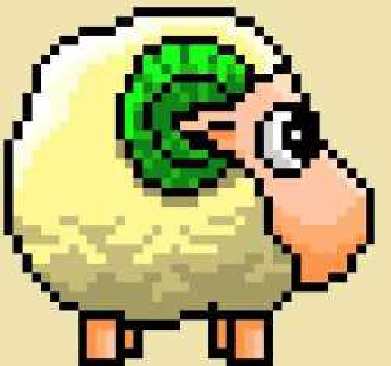
\includegraphics[width=0.75\textwidth]{kuvaesimerkki.pdf}
\caption{Kuvan elementit.}
\label{kuvaesimerkki}
\end{center}
\end{figure}


Kuvien kokoon on kiinnitettävä huomiota. Käytettyjen merkintöjen
on oltava helposti luettavissa ja selkeät. Esimerkiksi
suorituskykykäyriä esitettäessä akselit on nimettävä, asteikot
merkittävä ja käytetyt yksiköt tuotava selkeästi esiin.
Samankaltaisia asioita esitettäessä useammalla kuvalla on
syytä käyttää samaa mittakaavaa vertailun helpottamiseksi.

Kuvan otsikko kirjoitetaan kuvan alle ja sen tulee olla mieluummin lyhyt
ja ytimekäs kuin liian selittelevä.
Samoin toimitaan taulukoiden otsikoinnissa.

Kuvat ja taulukot numeroidaan juoksevasti. Pitkissä teksteissä käytetään
kaksitasoista numerointia (esimerkiksi Kuva 3.1) pääluvuittain, lyhyissä
riittää yksitasoinen numerointi.


Kuva- ja taulukko-otsikoiden yhdenmukaiseen esitystyyliin on syytä kiinnittää
huomiota, samoin mm. välimerkkeihin. Luontevaa on käyttää
kuvatekstin lopussa pistettä, ovathan useimmat kuvateksteistä virkkeitä. 

(Kuvien ja taulukoiden otsikointityyli vaihtelee
kustantajittain ja julkaisuittain. Samoin tuntuu suositeltava käytäntö
Tietojenkäsittelytieteen laitoksen sisällä vaihtelevan taulukon
otsikon sijainnin suhteen.)


\section{Otsikot}

Otsikoissa voi käyttää muusta tekstistä poikkeavaa kirjasintyyppiä,
alleviivausta, suurempaa kirjasinkokoa tms.\ erotuskeinoa, yleensä
kuitenkin vain yhtä näistä, koska kovin monta erilaista kirjasintyyppiä
ja -kokoa tekee ulkoasusta helposti sekavan.  Otsikoiden esitystavan on
oltava johdonmukainen läpi koko kirjoituksen. Numeroimattomia
''ylimääräisiä'' otsikoita ei tule yleensä käyttää.


\section{Mallin käyttö}

Voit käyttää tätä kirjoitusta mallina oman opinnäytteesi ulkoasua
varten. Eri tekstinkäsittelyjärjestelmissä käytössä olevat yksityiskohdat kuten
kirjasintyypit ja -koot ja rivivälit  poikkeavat toisistaan, joten
pienet poikkeamat ovat toki hyväksyttäviä.

Tieteellisen kirjoittamisen kurssin luennoilla ja
liitteenä olevassa ohjeessa annetut töiden ohjeelliset sivumäärät
koskevat työtä, joka vastaa ulkoasultaan tätä ohjetta (kirjasinkoko
12~pistettä). Tässä tekstissä keskimääräinen rivin pituus lienee noin
80~merkkiä ja sivun pituus 35-40~riviä.
Sivumääriin lasketaan varsinaisen tekstiosuuden pituus ja lähdeluettelo
(arabialaisin numeroin numeroitu osuus), ei kansilehteä, tiivistelmää
eikä sisällysluetteloa. Sivumääräarviossa otetaan huomioon hyvin vajaat
sivut, joita syntyy paljon lyhyiden lukujen ja taittotyyliin määritellyn
luvun avauksen pakottaminen oikeanpuolimmaiselle sivulle. 

\chapter{Yhteenveto}

Tämän kirjoituksen tarkoituksena on toimia muistilistana eräistä
esitystavallisista säännöistä, joihin harjoitusten ja tutkielmien
kohdalla on syytä kiinnittää huomiota.

Annetut ohjeet on laitoksen henkilökunta muotoillut yhdessä keskustellen
ja noudattaen oman tieteenalansa perinteitä. Eri erikoistumisaloilla ja
erilaisillaa määräävässä asemassa olevissa julkaisufooruilla käytänteet
vaihtelevat ja nuorten tutkijoiden onkin tiedostettava ero yleisten
sisältöohjeiden ja teknisten muotoilusääntöjen välillä. Aina tekstin
valmistuessa on tarkastettava erikseen, täyttääkö se annetut
pituusrajoitteet ja vastaako se annettuja muotoiluohjeita, olivatpa ne
kuinka pikkutarkkoja tahansa. Tarkasta sääntöjen noudattamisesta syntyy
yhteinäisyyttä kokoovan julkaisun tasolla, mikä helpottaa lukijoiden
työskentelyä.

Tämä ohje vastaa vain asettelullisiin kysymyksiin ja sen rinnalla on
syytä tutustua materiaaliin ja luentoihin, joissa keskitytään tekstin
varsinaiseen sisältöön. Olennaisin väline on kuitenkin akateemisesti
pidemmälle ehtineen, jo julkaisuja rakentaneen ohjaajan palaute ja
mentorointi.


%%
\chapter{Introduction}


In all writing for publication, the writer's freedom of creation and expression are limited by a number of guidelines and specific regulations.

At best, a familiar set of regulations shared by reader and writer can create a kind of support network that allows the message to be relayed without distortion. It will be easier for readers to find 
the pertinent contents in a piece of writing if its layout and structure are the same as they are used to. This also applies to writers. When writers follow a set presentation model, 
they do not have to waste time on considerations that are secondary to the work itself, but they can concentrate on polishing the contents of the text. This means that it is a good 
idea to practice following the rules for the layout, though you may think you know how to select a better way to present your work.

This is a guide for the layout and structure of theses and essays at the Department of Computer Science at the University of Helsinki. It is thus applicable to the course 
Scientific Writing, the software engineering projects, seminars, and MSc theses. (This is an updated version of 
the previous guide written by the course lecturers \citep{erkio01, erkiomakela96, erkio94, verkamo92}.)

The \LaTeX\ guide and \LaTeX\ style that has been  published on the department's web site can be used as support for this guide.


\chapter{Structure}

Let us start by looking at the sections expected to be in a scientific text. Keep in mind that the same expectations go for all kinds of technical writing.
However, this document in itself, is not a scientific or a research
text, so there will be content lacks in terms of research question
setting in the introduction and evaluative material in the last sections.

\section{Abstract or summary}
%\enlargethispage{5mm}


The summary page contains the following elements: the bibliographical data of the work, an abstract, topic classification, 
and the key words. The bibliographical data consists of title, name of the author, place of publication, date of publication, and number of pages.

The abstract should be short, generally one paragraph (100 words maximum) explaining the main contents of the work: topic, methodology and results.


 Topics are classified according to the ACM Computing Classification System
(CCS). A small set of paths (1-3) should be used, starting from any top nodes
referred to bu the root term CCS leading to the leaf nodes. The elements
in the path are separated by right arrow, and emphasis of each element individually can be indicated
by the use of bold face for high importance or italics for intermediate
level. The combination of individual boldface terms may give the reader
additional insight. 

\section{Introduction}


The purpose of the introduction is to introduce the goals of the work in general terms. Describe topic, 
methodology and results (as in the abstract, but expand it).
In order to provide the reader a good starting point for
interpretations, it is good to start the introduction by
contextualisation of the challenges and solutions to be discussed. For
example, why a certain domain has a particular challenge and who are
intended to benefit from the solutions proposed.

The length of the introduction depends on the length of the whole work. A few pages of text does not need a 
separate introduction, since it is an expanded summary in itself. The introduction to a 10-page text can 
be 1--1.5 pages long. For a 50--70-page MSc thesis, a 2--4-page introduction seems reasonable.

The introduction should shortly describe the problem field of the whole work, the plot, and the conclusions, 
in general terms. After reading it, the reader may decide whether to go deeper into the topic by reading the whole text.


\section{Topic chapters}

The nature of the matter at hand determines how the topic chapters are disposed.
In order to guide the reader, it is a good idea to start each main chapter with a short paragraph 
on what the main topic of the chapter is and how it progresses from one sub-chapter to the
next. Especially relevant is to express how concepts, challenges,
solutions and research steps are bound together. There should be enough
guidance for the reader to allow expectation of the right storyline.


Basic rule for easy to follow text is to use the natural emphasis of the
text structure to support the content matter key concepts and thought
processes. This means using openings of sectiosn and text paragraphs for
key arguments and information moves, while the internal parts of
paragraps are filled with supporting aspects that those less familiar
with the topic area need. Those with better background knoweldge can
quickly skim trhough the text without loosing any essential arguments.

Each author has his or her personal ryhtm in the text, which is visible
for the reader as the length of text paragraphs and complexity of
thought chains within. A good policy is to take only one information
move or transition per paragraph. This way the text stays easy to follow.

Signs of problems with the disposition of the text are easily seen in texts
with only one sub-chapter, or with more than two chapter levels (main and sub-chapters). There may be justifiable reasons to use three-level 
headings in some technical documents. Single sentence text paragraphs
are also to be avoided.



%\pagebreak
\section{Reference usage}


Relevant learning targets include superficial knowledge of several
citation styles and capability (and willingness) to follow a given
style and ordering of entires and bibliographical details in the list of references.
These aspects are essential as the approval of a PhD manuscript or
journal article may depend on them.

Disregard of which style you use, 
references are always placed inside sentences.  This means that e.g. a separate reference at the end of a paragraph would be inappropriate.

The structure of the text must clearly show what the reference relates to.  At the same time, it 
shows how long a piece of the text that the reference relates to.

Efficient positions for citations are right after the introduction
(definition) of a concept, a methods or such, or in the end of a claim
from the reference material. Furthermore, if quoting verbatime one must
use citation marks.

The text structures and wordings, in addition to the location of
ciations must clearly express whether claims or arguments are 
authors' own, or if they come from the contribution of others. Thus is
is of bad style to open a section by listing the citations on which the
section is based on. Such method can further indicate more serious
problems like following reference material as it is instead of analysing
and synthetising material into new though processes. 


\section{Conclusion}

At its simplest, a conclusion is merely a weak revision of the main points of the text.  All more valuable 
conclusion sections contain comments on e.g. the value of results, how the work relates to its environment, or 
future visions. This kind of evaluations should be well-grounded in fact, though, or the conclusion 
might inadvertently seem comical. 

\section{Creating the list of references}

The following guidelines should be followed when creating lists of reference for the 
assignments during the course Scientific Writing.

The guidelines are backed by two main goals: to make it as easy as possible to find the 
referenced source, and to show what kind of evaluation process the referenced work has undergone. For these reasons
\begin{itemize}

\item the reference notes should always be so exact that the source can be recognized and found in catalogues and libraries

\item different types of sources (monographs, conferences, journals) have to be easy to distinguish from each other, and 

\item the different parts of the list must conform to each other, especially for each source type.
\end{itemize}


Independent of the citation style in use, 
the sources are listed alphabetically according to the author's name, and works by the same 
author (group of authors) in the order in which they have been published. If some publication 
does not have an individual writer, it is alphabetized according to its name.


The following information should be given on each source independent of
the citation style:
\begin{itemize}
\item
Name(s) of author(s) (surname, initial letters of first names) in the original order; if there are more 
than three authors, we can write the name of the first author and {\em et al.} instead of the other names.

\item
the name of the publication or article in its original form

\item
place of publication:

\begin{itemize}

\item
of monographs: publisher, place of publication (can be omitted if the publisher is well known), year
\item
of journal articles: name of journal, volume, issue, year and month (in parenthesis)

\item
of articles from article collections (such as conference publications):
\begin{itemize}

\item name of collection, editor, publisher, place of publication and year 

{\em or}

\item conference name, coordinator, place and time,

\end{itemize}

\item
of a report: series, report number, place, publisher and year

\item
of a web source: URL, validity date, possibly the date when referenced in square brackets

\end{itemize}

\item
page numbers, if the source is an article or constitutes a chapter in a compilation.
\end{itemize}


When using web sources, you should keep in mind that the threshold for publication on the web 
is non-existent. It is better to concentrate on the publications of well-known scientific 
publishers and the technical standards for which the web is the only publication channel. If 
the same publication is available on paper, refer to that primarily and add the URL as a complement.


The list of references gives an example of a text that has been published through many 
channels~\citep{abiteboul,dietinger}and another example that shows a standard that has 
been disseminated only through the web~\citep{bray}. For web-based
references it is important to give both the publication date and the
time of reading and interpreting the material. The content is prone to
change, and dating your use, you protect your interpretations for
unnecessary accusations of being faulty, if it is known which version
you used.



The list of references for a text should list exactly the sources that the text refers to. 
The list of references for this text is an example of how to present sources, 
which is why it contains ''extra'' sources.


In any style,
put a full stop after the name of a publication or article, as well as after the bibliographical 
data of each reference. Separate the other pieces of information with a comma. As is normal in 
Finnish, only the first letter of the first word in the heading is capitalized, but in the titles of 
conferences and compilations, each major word is capitalized (not articles or prepositions). See the 
appended example for a model. For the sake of clarity, it is best to write {\em In the work} before 
the name of a compilation, except in the case of conference publications where the name starts with 
the abbreviation {\em Proc.} (for Proceedings). In such cases, no complement is necessary. You can 
see the difference by comparing the layouts of the references ~''\citep{dantowsley90}'' and~''\citep{gannonetal89}'' .
In case of other citation styles, it is likely that you can trust the
results given by the automated reference management tools.

\chapter{Layout}

This chapter discusses the main issues of the technical presentation of a text.


\section{Disposition of text sections}


Each text should include a separate cover page, as in this model. The second page contains an 
abstract, followed by a table of contents (on one or more pages), and then the main text.  
Pagination starts on the first page of the main text (with the Arabic numeral 1). (Rigorous writers 
leave out the number from the first page.) All the (numbered) headings and their page numbers should be 
written into the table of contents. Many word-processing systems create the table of contents automatically 
so that the writer does not have to worry about updating page numbers as the work progresses. If writers 
wish to, they can paginate the table of contents and previous pages separately (with Roman numerals), e.g. like this model.

After the main text, but as part of the text body, comes the list of references; its heading is 
not numbered. Any possible appendices are added after the list of references, with headings and internal page numbers.

%\enlargethispage{5mm}

If you want to make a coherent list of figures, algorithms and tables, this list should be placed i
mmediately after the table of contents. The value of such lists is a matter of opinion, so there 
is no need to create one --- especially if your word-processing software does not support it --- unless your instructor explicitly asks for it.

If for some special reason you want to add an alphabetical index top your work, it should be placed after 
the list of references and before appendices. An index should be noted in the table of contents, as s
hould the list of references (unnumbered chapter). Writers who want to create an index should use the automatic support their word-processing system offes.

\section{General text layout}

Nowadays you may plan your text to be printed on single side or double
side, with line spacing one, for the final copy.

For reviewing and feedback purposes, check with your readers for their
preferences. Most read and comment on paper and need some space for
marking. 
For drafts you can use wide margins too. 
Both margins should also be fairly broad (ca.~3~cm): the wider left margin is needed for binding the text and the
right one for the instructor's comments.  Leave enough space (2--3~cm) at the top and bottom, as well.

The most effective way to distinguish features like chapters, figures, etc,  is to have enough space 
in your text.  Separate paragraphs from each other with one and chapters with a few empty lines.  If a 
new chapter is about to start at the bottom of a page (with only one or two lines of text), it is better 
to start it on the next page.  However, it is not necessary to start every chapter on a new page, especially 
not with a short text; if the text contains many pages that are nearly empty, readers might suspect that the 
writer has tried to make it look longer than it is.


Any empty space may be utilized for displaying figures and tables.  Especially if a text is written with the 
same type of text throughout, empty lines are necessary for separating e.g.~text from tables.  Empty space 
is cheap, but adds to the clarity and readability of a text.

\section{Figures and tables}

%\enlargethispage{5mm}

All figures and tables should be placed as near the (first) place in the text that refers to them, but 
not before this reference. The text should also explain what the writer wants to illustrate with the 
figure. Figures can be interpreted in many different ways, so the reader needs guiding.

Figures should never be placed immediately under the heading of a chapter, but chapters should always 
start with text. Figures should not be placed in the middle of a paragraph (much less a sentence), except 
if the figure is placed at the top or bottom of a page and it is clear that the paragraph continues.

Figures do not always have to be placed immediately after the paragraph that refers to them. If there is 
not enough space for a figure on the same page as the paragraph that refers to it, the rest of the page 
should not remain empty, Though the figure is inserted on the following page. However, the figure should 
never be more than one page away from the reference.


The image~\ref{kuvaesimerkki} shows how to present a figure. You must pay attention to the visibility of 
figure parts and text, to the numbering of figures, and captions. 

\begin{figure}[ht]
%\begin{figure}[tbh] t= top, b = bottom, h=here
\ \newline
\begin{center}
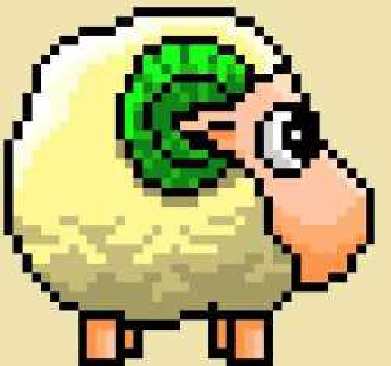
\includegraphics[width=0.9\textwidth]{kuvaesimerkki.pdf}
%\rotatebox{90}{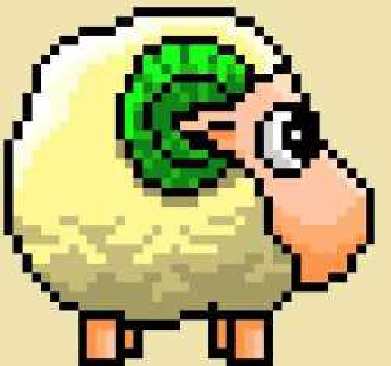
\includegraphics[scale=.75]{kuvaesimerkki.pdf}}
\caption{Figure elements.}
\label{kuvaesimerkki}
\end{center}
\end{figure}


We must also pay attention to the size of figures. Any annotations must be clear and easy to read When 
presenting performance curves, for example, the axels have to be named, the scale notated, and the units 
clearly presented. If you present many things with similar figures, you should use the same scale for easy comparison.

The caption of a figure should be written underneath it, and it is preferable that it be short and to 
the point than too explicit. The same goes for table captions.

Figures and tables should be numbered progressively. In long texts, two-level numbering should be 
used (e.g. Figure 3.1) according to the chapter number, but in shorter texts, one-level numbering is good enough.


You should pay attention to presenting figure and table captions consistently, as well as to punctuation 
marks. It is natural to put a full stop after a caption, since they are most often full sentences. 

(The style for figure and table captions vary according to publisher and publication. The recommendations 
at the Department of Computer Science also seems to vary with respect to where the caption should be placed.)


\section{Headings}

You can use a different font in headings than in the rest of the text, or underlining, larger fonts, or other 
methods of emphasis, but generally it is preferred that you only use one of these methods, because if there are 
very many font types and sizes, the layout looks messy.  The format of headings must be consistent throughout 
the text. You should not use any unnumbered ''extra'' headings.


\section{Using this model}

You can use this text as a model for the layout of your own assignment. The font types and sizes, 
line spacing, etc vary according to word-processing system, so small deviations from the rule are acceptable.

The directive number of pages for written assignments given during the lectures for the Scientific-writing 
course and in this guide are applicable to assignments with a layout like this guide's (font size 12 points). The 
average line in this text should consist of about 80~characters and one page about 30~lines. The number of pages 
includes the text itself and the list of references (the part paginated with Arabic numbers), not the 
cover page, summary, or table of contents.

\chapter{Conclusion}

This text is a checklist for some of the rules governing written presentations, which you should 
keep in mind when writing exercises and theses.

This collection of advise has been compiled by staff members as the
result of discussions on general good writing habbits in computer
science. The consensus is that all young researchers and academic degree
holders must be able to seek and follow instructions of layout and
structuring of texts depending on the contribution they are working on. 
This set of instructions aims at unifying the looks of theses and other
study reports from the department, but it is also a representative of
the instruction sets students will meet later.

This set of instructions only address the looks of the document. Other
instructions must be sought, read and gained experience with in order to
learn to select the suitable semantical contents for the scientific texts.



\end{appendices}
%%%%%%%%%%%%%%%%%%%%%%%%%%%%%%%%%%%%%%%%%%%%%%%%%%%%%%%%%

\end{document}
